\documentclass[11pt,a4paper]{report}
% Aberstwyth dissertation LaTeX Template
% Authors: Dr. Hannah Dee (hmd1@aber.ac.uk), Neil Taylor (nst@aber.ac.uk)
% This has been adapted from the Leeds Thesis template and the 
% Group Project template for Computer Science in Aberystywth University.
% 
% All comments and suggestions welcome.
%
% Template designed to be used with pdflatex: it may need alteration to
% run with a different LaTeX engine.
%
% Note - this is offered as a starting point for your work. You are not 
% required to use this template and can choose to create your own document 
% without it. 

% To build document on the unix command line, run four commands:
 
% pdflatex dissertation
% bibtex dissertation
% pdflatex dissertation
% pdflatex dissertation
%TC:group tabular 1 1
% you will end up with dissertation.pdf 
\usepackage{mmp}
\usepackage{longtable}
\usepackage{lscape}
\usepackage{pdflscape}

% the following packages are used for citations - You only need to include one. 
%
% Use the cite package if you are using the numeric style (e.g. IEEEannot). 
% Use the natbib package if you are using the author-date style (e.g. authordate2annot). 
% Only use one of these and comment out the other one. 
\usepackage{cite}
%\usepackage{natbib}

% Allow up to 4 levels of nesting of sub-sub sections
\setcounter{secnumdepth}{4}

% Use the following to selectively exclude chapters
%\includeonly{cover,abstract,acknowledge,declare,chapter1,chapter2}

\begin{document}

\captionsetup{justification=centering}

% all of the include directives below refer to tex files
% so \title{Aber Fitness Project}

% Your names
\author{Adam Lancaster [arl4], Andrew Edwards [ane18], Charlie Lathbury [ckl2], Daniel Monaghan [dkm2], David Fairbrother [daf5], Jack Thomson [jat36], James Britton [jhb15], Robert Mouncer [rdm10]}

\modulecode{SEM5640} % i.e. CS39440, CC39440, CS39620
\moduletitle{Developing Advanced Internet Based Applications} % i.e. Major Project or Minor Project

\date{\today} % i.e. the date of this version of the report

\status{Release} % Use draft until you create the release version. Then, change this to Release.
\version{1.0.1}

\maketitle



 includes cover.tex - to change the content,
% edit the tex file

\pagenumbering{roman}

% This is the front page
\title{Aber Fitness Project}

% Your names
\author{Adam Lancaster [arl4], Andrew Edwards [ane18], Charlie Lathbury [ckl2], Daniel Monaghan [dkm2], David Fairbrother [daf5], Jack Thomson [jat36], James Britton [jhb15], Robert Mouncer [rdm10]}

\modulecode{SEM5640} % i.e. CS39440, CC39440, CS39620
\moduletitle{Developing Advanced Internet Based Applications} % i.e. Major Project or Minor Project

\date{\today} % i.e. the date of this version of the report

\status{Release} % Use draft until you create the release version. Then, change this to Release.
\version{1.0.1}

\maketitle



               

\setlength{\textwidth}{7in}
\setlength{\oddsidemargin}{-0.4in} \setlength{\evensidemargin}{0in}         

% Set up page numbering
\pagestyle{empty}

% declarations of originality 
\thispagestyle{empty}

%TC:ignore

%%%
%%% You must sign the declaration of originality. 
%%%
%%% You are submitting this electronically. Therefore, to sign, you 
%%% type your name and date to replace the .... characters. 
%%%
\begin{center}
    {\LARGE\bf Declaration of originality}
\end{center}

We confirm that:

\begin{itemize}
\item{This submission is our own work, except where 
clearly indicated.}

\item{We understand that there are severe penalties for Unacceptable Academic Practice, which can lead to loss of marks or even the withholding of a degree.}
 
\item{We have read the regulations on Unacceptable Academic Practice from the University's Academic Registry and the relevant sections of the current Student Handbook of the Department of Computer Science.}
 
\item{In submitting this work we understand and agree to abide by the University's regulations governing these issues.}

\end{itemize}


\begin{tabular}{|l|l|}
\hline
\textbf{Name} & \textbf{User ID} \\
\hline  
  Britton, James  	 	&  jhb15 \\
  Edwards, Andrew  		&  ane18 \\
  Fairbrother, David    &  daf5  \\
  Lancaster, Adam 		&  arl4  \\
  Lathbury, Charlie		&  ckl2  \\
  Monaghan, Daniel		&  dkm2  \\
  Mouncer, Robert		&  rdm10 \\
  Thomson, Jack			&  jat36 \\
\hline       
\end{tabular}

\vspace{1em}
\textbf{Date:} December 2018 \\

%TC:endignore               

\pagenumbering{roman}
\pagestyle{fancy}
\fancyhead{}
\fancyfoot[C]{\thepage}
\renewcommand{\headrulewidth}{0 pt}
\renewcommand{\chaptermark}[1]{\markboth{#1}{}}

\tableofcontents   
\newpage
\listoffigures
\newpage 

% Set up page numbering
\pagenumbering{arabic}

\setchapterheaderfooter

% include the chapters
\chapter{Overview}

\begin{center}
	
\includegraphics[width=0.5\textwidth]{Images/aberfitness.png}
\end{center}

\par
\textit{Aber Fitness} is a web application developed using Microsoft's \textit{.NET Core} and Oracle's \textit{Java Enterprise Edition} (henceforth referred to as Java EE). The project aims to provide a service which encourages fitness and promotes engagement with sporting activities amongst the users of the application, by offering functionality such as:

\begin{itemize}
	\item Graphing fitness data gathered by owners of \textit{Fitbit} devices, or through manual input.
	\item The ability to take part in challenges based on that fitness data.
	\item Providing a Sport ladder system, which has tight integration with a bespoke facility booking system.
\end{itemize}

\textit{Aber Fitness} aims to offer everything that would be needed by a sporty and active person in order to bring their sporting activities onto a digital platform and also to enhance their use of devices they already own, such as \textit{Fitbit} devices or smart watches such as the \textit{Apple Watch}.

\par
At launch, the system will ingest activity data automatically from \textit{Fitbit}, and be open to the addition of other health data provider services at a later date due to the modular nature of the data ingest system. Once normalised, this activity data will be used throughout the various microservices within \textit{Aber Fitness}, providing users with functionality such as a dashboard overview of their activity over the past month, as well as integrating tightly with the challenges microservice to add a competitive aspect to the system, with the aim of keeping users engaged with both the platform itself and keeping fit in general.

\par
Aber Fitness will also feature a number of supporting tools, such as:

\begin{itemize}
	\item A user management system with two-factor authentication.
	\item A comprehensive audit trail of when and how their data was used and accessed, which is filterable by date.
	\item A global layout template with a dynamic sidebar, which can be adjusted by administrators. Those changes will be instantly propagated to the other microservices.
\end{itemize}

\par
\textit{Aber Fitness} will also be designed to be scalable and easily deployed through the use of \textit{Docker}, by segregating related functionality into individual microservices.

\label{Requirements_chpt}
\chapter{Requirements}

A list of functional requirements was provided by the client when the project began. As the project progressed, these were clarified and refined using \textit{Slack}\cite{slack} as a channel of regular communication with the client. The following tables detail the areas in which the final set of requirements differ from those provided at the start.

\section{Data Gathering and Storage}
\begin{tabular}{ |p{5cm}|l|l|p{8cm}|}
\hline
\textbf{Requirement}	&	\textbf{FR\#}	&	\textbf{Completed}	&	\textbf{Comments} \\
\hline
Management of Participants in the System			& DG-FR1	& Yes	&  Clarification with the client confirmed that a member can only be associated with one group. \\
\hline
Activity Data										& DG-FR2	& No	&  \\
\hline
Linking a participant to a server-based data source	& DG-FR3	& Yes	&  \\
\hline
Obtaining data from the server-based data source	& DG-FR4	& Yes	&  \\
\hline
Receiving data from other devices					& DG-FR5	& Yes	&  \\
\hline
Receiving manual input of data						& DG-FR6	& Yes	&  \\
\hline
Data to retrieve 									& DG-FR7	& Yes	& Additional requirement - All step data should be collected for the system. This will include "workout" sessions. \\
\hline
Removing data for a participant						& DG-FR8	& Yes	&  Requirement complete. \\
\hline
Administrator access to data						& DG-FR9	& Yes	& The client confirmed that the administrator should be able to edit all individual readings for a user (whether from Fitbit or manual entry).\\
\hline
Activity data management							& DG-FR11	& Yes	& Additional requirement - An interface should be provided for the administrator to map \textit{Fitbit} activities onto the activities created for the system. \\
\hline
\end{tabular}

\section{User Management}
\begin{tabular}{ |p{5cm}|l|l|p{8cm}|}
\hline
\textbf{Requirement}	&	\textbf{FR\#}	&	\textbf{Completed}	&	\textbf{Comments} \\
\hline
Authentication and authorisation 					& UM-FR1 	& Yes 		&  \\
\hline
Local User Accounts 								& UM-FR2 	& Yes 		& Additional requirement - The user accounts do not need to be Aberystwyth University integrated. Local user accounts should be used. \\
\hline
User Characteristics								& UM-FR3	& Yes		& Requirement specified in document but not given a functional requirement number. There will be three different types of users: member, coordinator and administrator. \\

\hline
\end{tabular}



\section{Health Dashboard}
\begin{tabular}{ |p{5cm}|l|l|p{8cm}|}
\hline
\textbf{Requirement}	&	\textbf{FR\#}	&	\textbf{Completed}	&	\textbf{Comments} \\
\hline
Review data for a member 							& HD-FR1 	& Yes 		&  \\
\hline
Set goals and view progress. 						& HD-FR2 	& Yes		&  \\

\hline
\end{tabular}


\section{Challenges}
\begin{tabular}{ |p{5cm}|l|l|p{8cm}|}
\hline
\textbf{Requirement}	&	\textbf{FR\#}	&	\textbf{Completed}	&	\textbf{Comments} \\
\hline
Create a challenge 									& C-FR1 	& Yes 		&  \\
\hline
Join a challenge 									& C-FR2 	& Yes  		&  \\
\hline
Activity during a challenge							& C-FR3 	& Yes 		&  \\
\hline
Closing the challenge								& C-FR4		& Yes 		&  \\
\hline
Types of challenges 								& C-FR5 	& Yes		& Additional requirement - There should be two types of challenge. "Personal goals", which are individual challenges, and "Group challenges", which are challenges created for members of a specific group to join. \\

\hline
\end{tabular}


\section{Booking System}
\begin{tabular}{ |p{5cm}|l|l|p{8cm}|}
\hline
\textbf{Requirement}	&	\textbf{FR\#}	&	\textbf{Completed}	&	\textbf{Comments} \\
\hline
Facilities      									& BS-FR1	& Yes      		&  \\
\hline
Availability   										& BS-FR2	& Yes      		& Requirement extended - An administrator block on a facility should be a single booking and not multiple hourly bookings. \\

\hline
Booking         									& BS-FR3	& Yes      		&  \\
\hline
Available Times 									& BS-FR4	& Yes      		& Additional requirement - A fixed time period for bookings should be available for a facility (9am - 9pm). \\

\hline
\end{tabular}

\section{Sports Ladder}
\begin{tabular}{ |p{5cm}|l|l|p{8cm}|}
\hline
\textbf{Requirement}	&	\textbf{FR\#}	&	\textbf{Completed}	&	\textbf{Comments} \\
\hline
Creating 											& SL-FR1	& Yes 		&  \\
\hline
Joining 											& SL-FR2	& Yes 		&  \\
\hline
Profile Update 										& SL-FR3	& Yes		&  \\
\hline
Suspension 											& SL-FR4	& Yes 		&  \\
\hline
Current Ladder	 									& SL-FR5	& Yes 		&  \\
\hline
View Member											& SL-FR6	& Yes 		&  \\
\hline
Challenge 											& SL-FR7	& Yes		&  \\
\hline
Scheduling 											& SL-FR8	& Yes 		&  \\
\hline
Response to a challenge 							& SL-FR9 	& Yes 		& Clarification with the client confirmed that the challenged user can suggest an alternative date-time and/or venue. \\
\hline
Expiry 												& SL-FR10 	& Yes		&  \\
\hline
Result 												& SL-FR11 	& Yes 		&  \\
\hline
Removal 											& SL-FR12 	& Yes 		&  \\
\hline
Match Involvement									& SL-FR13 	& Yes 		& Additional requirement - A member can only be involved in one match at a time. \\
\hline
Winning a match 									& SL-FR14 	& Yes 		& Additional requirement - If the loser of a match is in a higher position on the ladder than the winner, their position should swap with the loser. \\


\hline
\end{tabular}

\section{Engagement}
\begin{tabular}{ |p{5cm}|l|l|p{8cm}|}
\hline
\textbf{Requirement}	&	\textbf{FR\#}	&	\textbf{Completed}	&	\textbf{Comments} \\
\hline
Current Rankings 									& E-FR1		& No	& Some requirements have been met. After discussion with the client the requirement to have rankings between groups was changed to rankings within a group.  \\
\hline
Individual Progress									& E-FR2		& Yes	&  \\
\hline
Weekly Updates 										& E-FR3		& Yes	&  \\
\hline
Missing Reading Updates 							& E-FR4		& Yes	&  \\

\hline
\end{tabular}


\section{External Interface}
\begin{tabular}{ |p{5cm}|l|l|p{8cm}|}
\hline
\textbf{Requirement}	&	\textbf{FR\#}	&	\textbf{Completed}	&	\textbf{Comments} \\
\hline
Appearance & EIR1 & Yes. &  \\
\hline
Internationalised Interface & EIR2 & No &  \\
\hline
Handling UI - Proxy & EIR3 & Yes & Additional requirement - Services should generate their own UI, the UI should go back to the client via a proxy. \\
\hline
\end{tabular}

\chapter{Development Methodolgy}

\textcolor{red}{\textbf{TODO: Possibly restructure this, it\'s a start for now. Not 100\% sure what Neil\'s looking for here.}}

\section{Initial Project Plan}

Upon starting the project, we met as a group and decided on a standard style of development which would work best between all of us. After some discussion, we concluded that a \textit{Scrumban}\cite{scrumban} style of development would best fit our needs. Due to the relatively short duration of the project, and our team consisting of only eight developers, we decided on adopting this rather hands off development approach which focuses on flexibility and being able to change and adapt the project plan and sprints as the project progresses. The \textit{Scrumban} methodology was also suited to the project as the two technologies we were required to use, Java EE and .NET Core, were new to all of the members of our team, making estimating sprints and velocity quite difficult. 

We began the project by breaking the project specification down into disitinct microservices, and deciding which technologies would be best suited to each service. \textbf{TODO: Link to figure below}

\begin{figure}[H]
    \centering
    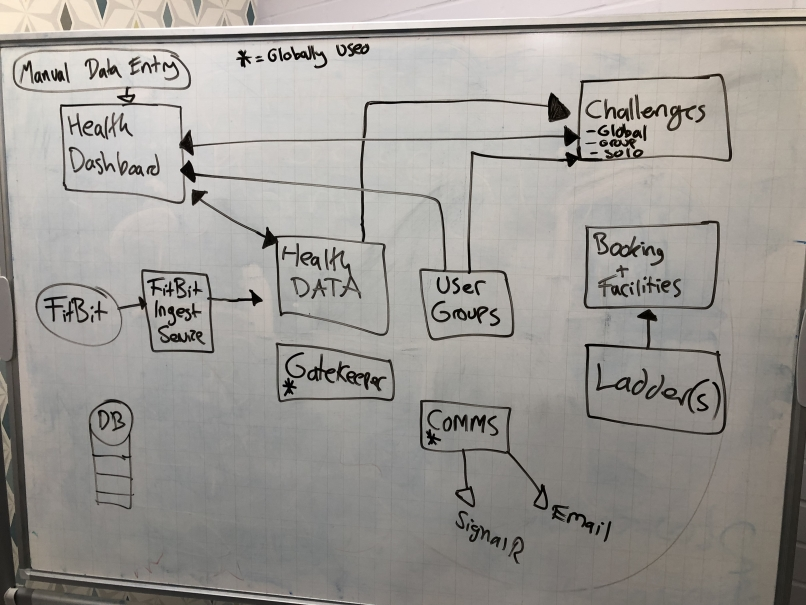
\includegraphics[width=\textwidth]{Images/Initial_Spec_Chart.jpg}
    \caption{An initial design diagram which was used to help break down the project into smaller microservices and gain a rough understanding how each microservice could interact}
\end{figure}

Once the individual microservices had been decided upon, we set out on allocating each microservice to two members of the team and assinging each service a priority ranking between 1 and 3, depending on how the services depended on one another. Services marked with a priority of 1 were core parts of the \textit{AberFitness} infrastructure on which many other parts of the system relied on their APIs in order to function correctly, such as the \textit{Health Data Repository} microservice.  \textbf{TODO: Link to figure below}

\begin{figure}[H]
    \centering
    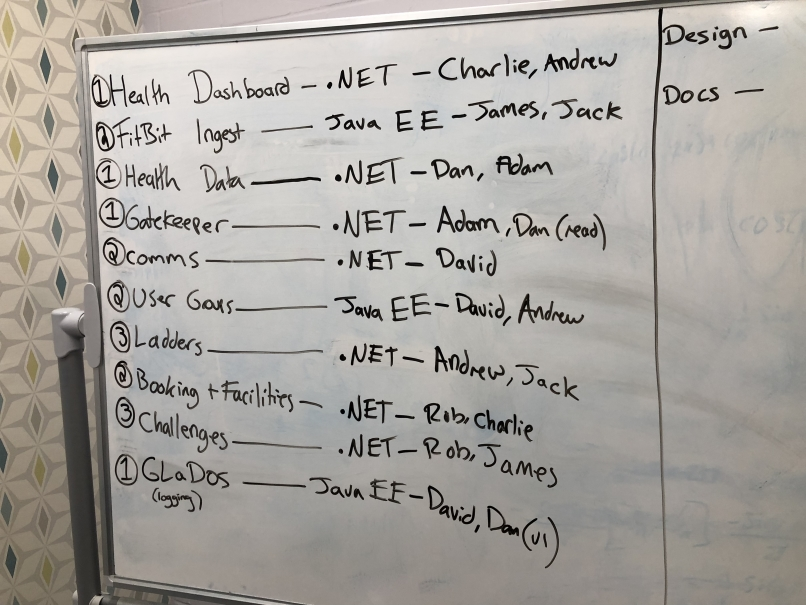
\includegraphics[width=\textwidth]{Images/Numbering_Microservices.jpg}
    \caption{Initial plan for ordering microservices in terms of priority and allocating them to members of the team for development}
\end{figure}


\section{Supporting Tools}
\subsection{GitHub \& TravisCI}
Each microservice for \textit{Aber Fitness} was hosted on \textit{GitHub}\footnote{https://github.com/sem5640-2018}. \textit{GitHub} provided many features which proved incredibly useful during the development phase, such as tight integration with \textit{Slack} for notifications straight to our chatrooms and integration with \textit{TravisCI} to automatically trigger unit tests and \textit{Docker} image builds. We also developed a development pattern of requiring all code to be peer reviewed through the use of pull requests and branch protection, a collection of settings which require that a series of conditions have been met before a pull request is able to be merged into the \textit{development} or \textit{master} branch. We configured branch protection in order to ensure that only tested, peer reviewed code would be committed into any upstream branch to reduce the likelihood of errors being introduced into the system and so that any issues could be caught early on. 

\begin{figure}[H]
    \centering
    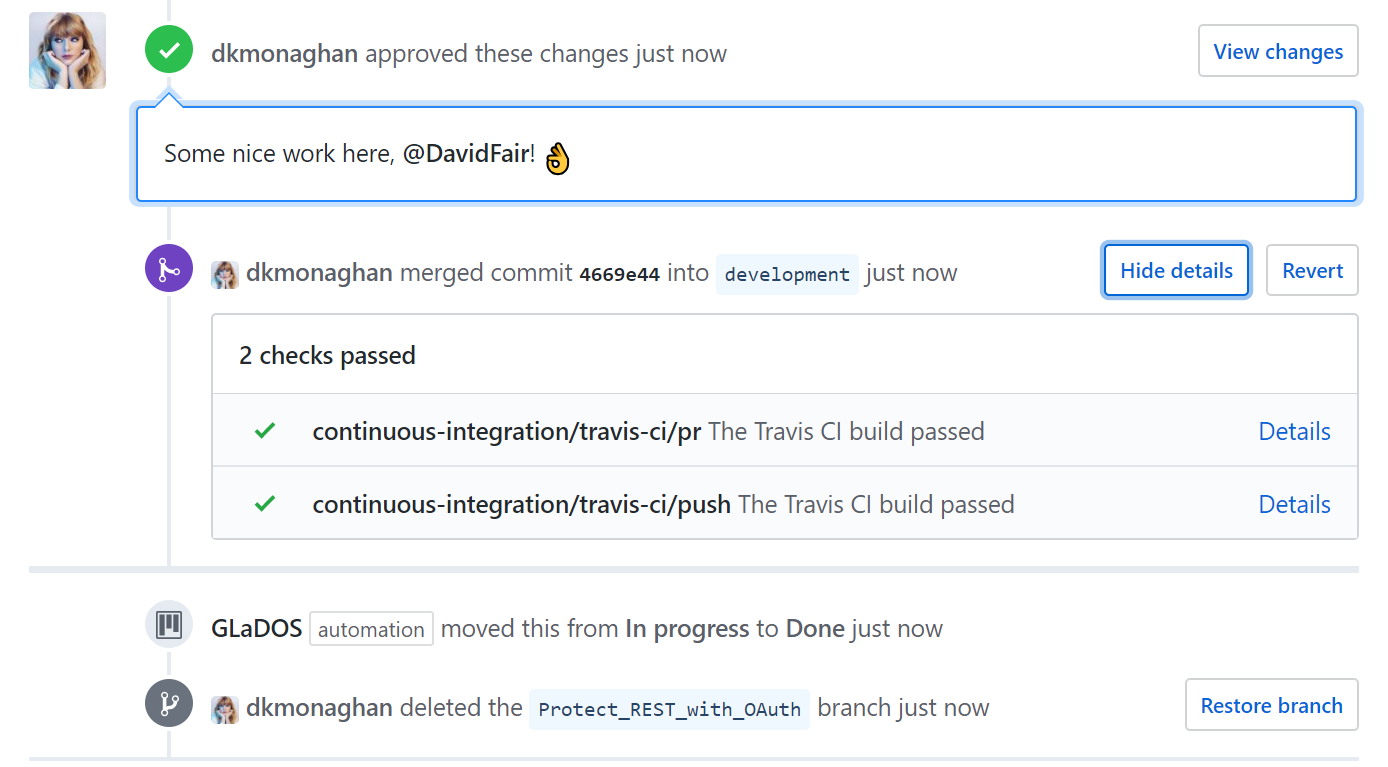
\includegraphics[width=\textwidth]{Images/approve_pr.png}
    \caption{A screenshot from \textit{GitHub} showing a pull request on the \textit{GLaDOS} repository being peer reviewed and also checks from \textit{TravisCI} passing before being merged into an upstream branch.}
\end{figure}

Once a pull request had been approved and merged, \textit{TravisCI} would then be responsible for building and pushing the \textit{Docker} image to \textit{Docker Hub}.

\begin{figure}[H]
    \centering
    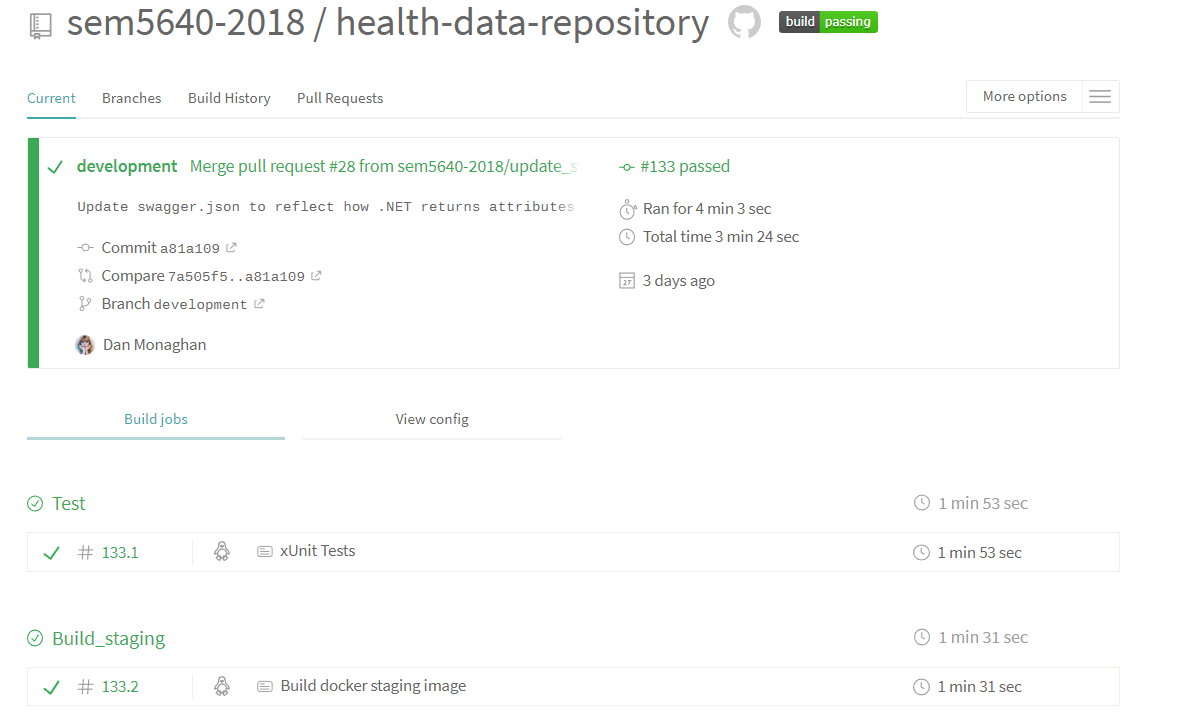
\includegraphics[width=\textwidth]{Images/travis_builds_overview.png}
    \caption{A screenshot from \textit{TravisCI} demonstrating a pull request being merged into the \textit{development} branch, re-passing unit tests once merged and then building the \textit{Docker} image}
\end{figure}

\subsection{Swagger}
\begin{figure}[H]
    \centering
    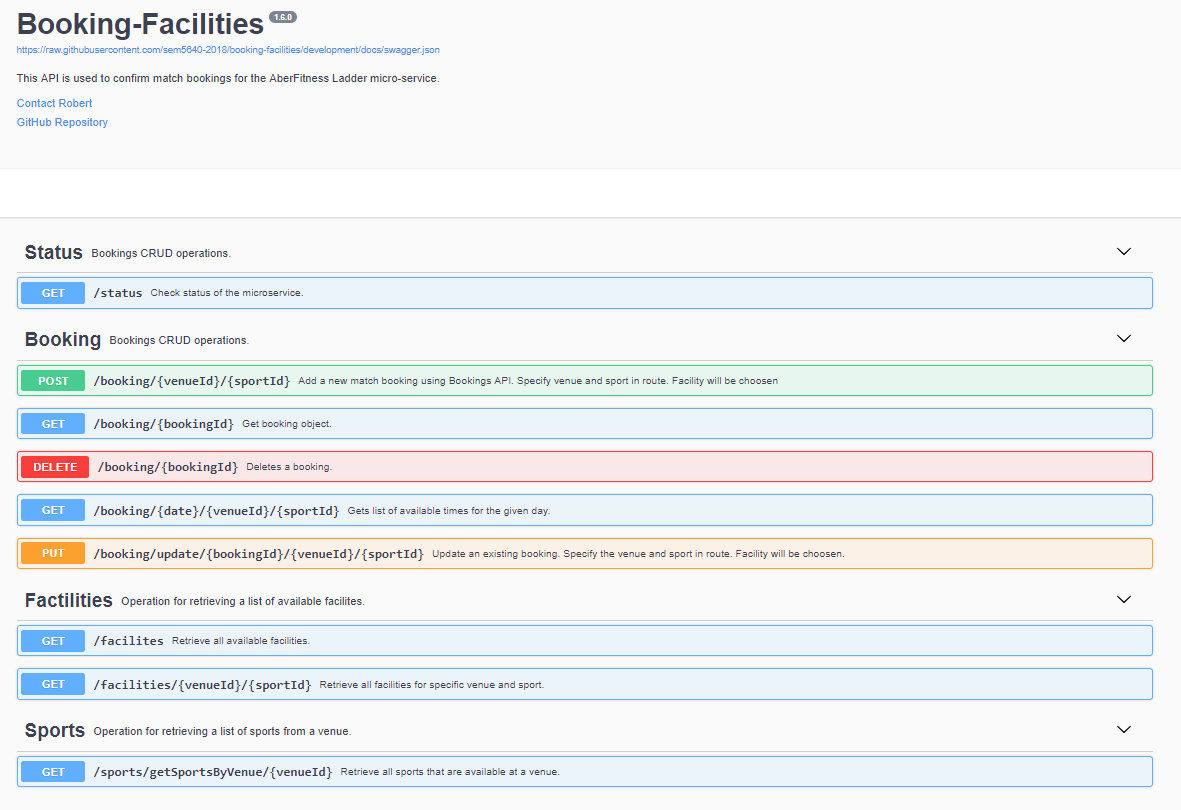
\includegraphics[width=\textwidth]{Images/Swagger.png}
    \caption{The Swagger interface for the \textit{Booking Facilities} microservice}
\end{figure}

\textit{Swagger} is a web based application for viewing API specifications. Each microservice within \textit{Aber Fitness} has a file located at \lstinline{docs/swagger.json} which defines its API endpoints and any associated data models. \textit{Swagger} was a crucial part of the development process as it allowed us to draft up API specifications prior to development in order to get feedback from other members of the group, and allowed issues to be identified early on in the event that a draft API specification lacked endpoints which would be required by other microservices. 


\subsection{Portainer}
\begin{figure}[H]
    \centering
    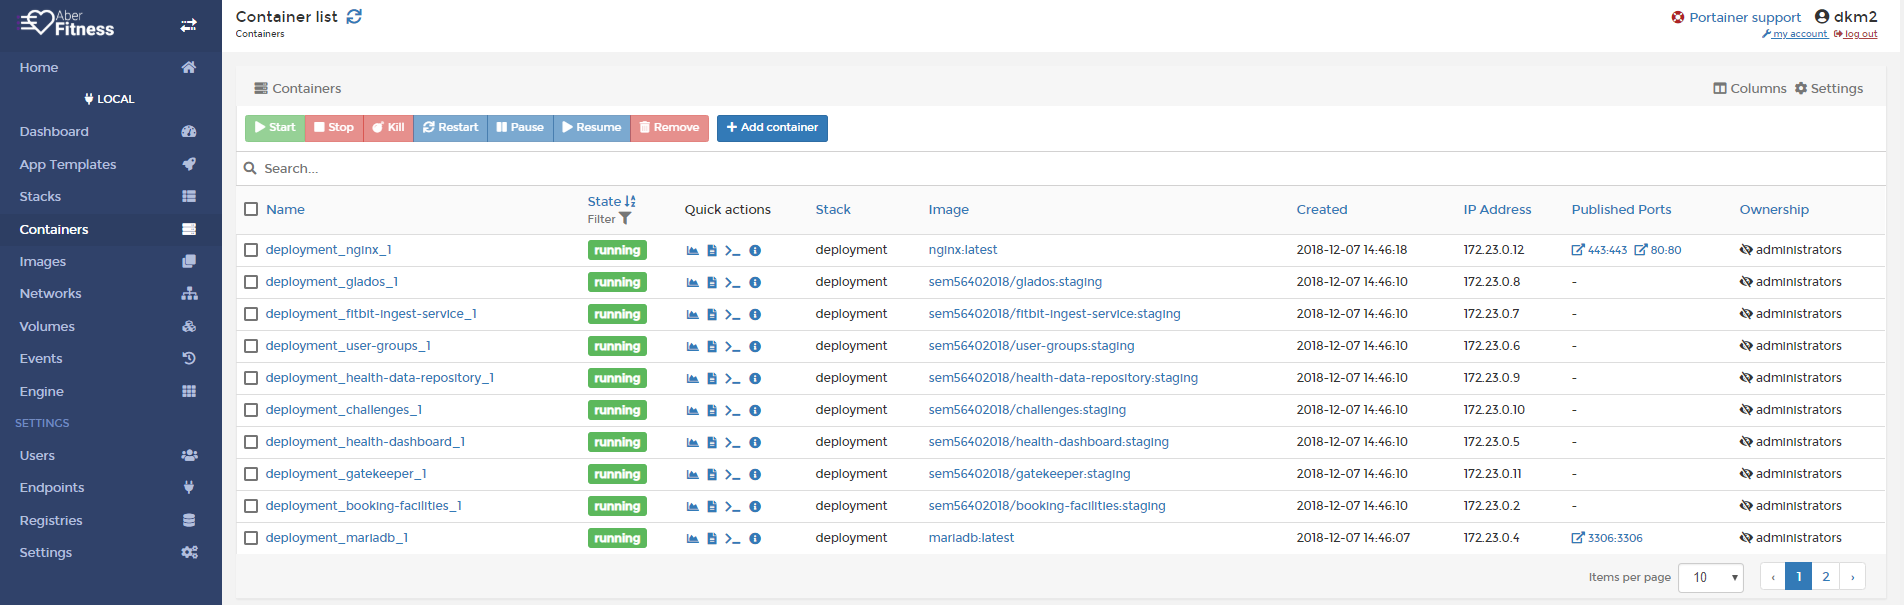
\includegraphics[width=\textwidth]{Images/Portainer.png}
    \caption{The Portainer interface for our staging / development Docker host, \lstinline{docker2-m56.dcs.aber.ac.uk}}
\end{figure}

\textit{Portainer} provides a dashboard for managing volumes, networks, images and containers on \textit{Docker} hosts. Throughout the initial configuration of the \textit{Docker} images, \textit{Portainer} proved invaluable as it provided the ability to quickly and easily understand what the host was running. \textbf{TODO: More here probably.}

\subsection{Docker Hub}
\textit{Docker Hub} is a platform provided by \textit{Docker} which allows \textit{Docker} container images to be uploaded and hosted, and easily pulled down by the \lstinline{docker-compose} script. As part of our build process (\textbf{TODO: reference build pipline diagram here}), images are built by \textit{TravisCI} and then pushed to \textit{Docker Hub} before being pulled down onto the \textit{Docker} hosts.


\subsection{Slack \& Deployment}
\textit{Slack} is an online text based chat service designed for offices and teams, and paticuarly suits itself to the development of software. The group used \textit{Slack} extensively throughout the development of \textit{Aber Fitness} not only to communicate and discuss progress, ideas and troubleshoot problems, but also made extensive use of \textit{Slack}'s integrations with services such as \textit{TravisCI} and \textit{GitHub}. 

\begin{figure}[H]
    \centering
    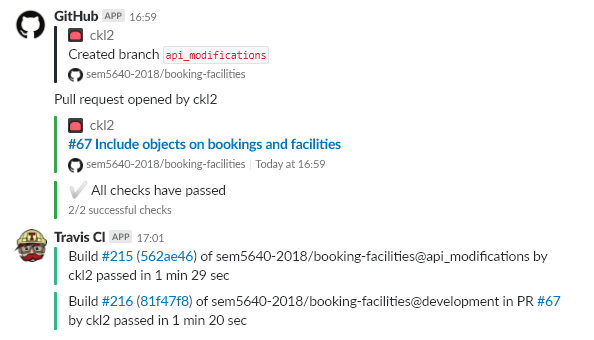
\includegraphics[width=\textwidth]{Images/Slack_Travis_GitHub.png}
    \caption{A screenshot of the \textit{Slack} channel \lstinline{\#dev-booking-facilities} demonstrating the integrations between \textit{Slack}, \textit{GitHub} and \textit{TravisCI}}
\end{figure}

\textit{Slack} also played a major role in our deployment strategy when rolling out updated \textit{Docker} images to our staging host. Due to the nature of the configuration of the two \textit{Docker} hosts we had been provided by the Computer Science department we ran into many issues with our deployment process, primarily to do with permissions on the host. Each member of the team had their own individual log in to the hosts, however we would frequently run into permissions errors when performing commands like \lstinline{git pull}. Other issues we had involved team members forgetting the specific set of commands which needed to be executed, wasting valuable development time. \textbf{TODO: figure no.}

\begin{figure}[H]
    \centering
    
\includegraphics[width=0.5\textwidth]{Images/aberfitness_slack_bot_reason_why.png}
    \caption{An example situation where the execution of \lstinline{docker-compose pull} caused a large amount of confusion amongst \textit{Aber Fitness} developers}
\end{figure}


\textit{Slack} ended up providing us with an elegant solution to this through its ability to easily call a webhook when a user typed a specific message in a chat channel. A quick \textit{Slack} application was put together to automatically pull the latest \lstinline{docker-compose.yml} file from GitHub, as well as updating all the \textit{Docker Hub} images, then re-deploying the stack. This could all be done from within \textit{Slack} itself through the \lstinline{/deploy} command. \textbf{TODO: Figure no.}

\begin{figure}[H]
    \centering
    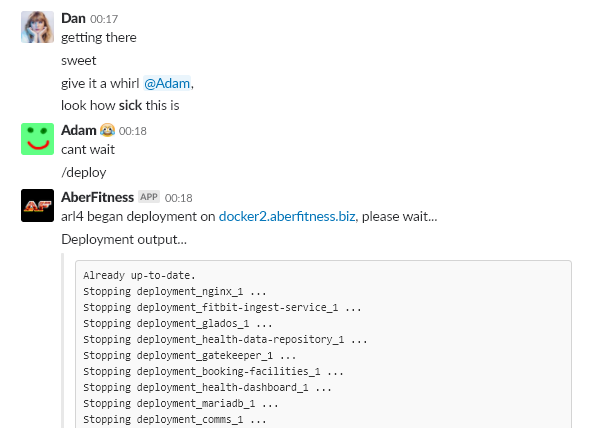
\includegraphics[width=0.9\textwidth]{Images/aberfitness_slack_bot.png}
    \caption{A demonstration of the \lstinline{/deploy} command being used to re-deploy \textit{Aber Fitness} onto the staging host}
\end{figure}


\chapter{Design}

\section{System Overview}
The \textit{Aber Fitness} system is broken down into a number of microservices in order to aid portability, scalability and promotes a more maintainable codebase. After reviewing the initial project specification, the following microservices were created:

\begin{itemize}

	\item \textbf{Booking \& Facilities} - The \textit{Aber Fitness} offers functionality for users to be able to schedule bookings at sports venues, such as swimming pools and squash courts. This microservice is called used by the \textit{Ladders} service to create bookings for competitions.

	\item \textbf{Challenges} - The system offers the ability to give users activity challenges, for example completing a number of steps in a specific timeframe. These challenges can also be 'group' challenges, where a number of users can compete against each another to achieve goals such as furthest distance walked in a week, etc.

	\item \textbf{Communications} - This microservice provides an API for other services to send email notifications to users. It does not present any form of web UI, and users do not directly interact with it. This system could also be easily expanded to send out text messages, push alerts, etc. depending on future requirements.

	\item \textbf{Fitbit Ingest Service} - At launch, the \textit{Aber Fitness} platform allows a user to link their \textit{Fitbit} accounts to the system in order to import their activity data. The service periodically polls the Fitbit API for new data on the users' behalf, then stores this into the \textit{Health Data Repository}.
	
	\par With the possibility of adding future platform support the "ingest service" concept was created. This would allow us to support services such as Apple's \textit{HealthKit} and other fitness tech providers. 
	This architectural design means that activity data can be normalised by a number of "ingest services" before being passed through to the \textit{Health Data Repository} service for storage. 

	\item \textbf{Gatekeeper} - \textit{Gatekeeper} is \textit{Aber Fitness}'s OpenID Provider, and handles all authentication within the system. User credentials and account metadata is stored within \textit{Gatekeeper}\textit{Gatekeeper} uses the OAuth 2.0 flow and is responsible for providing a single sign-on service for all of the various microservices. Microservices also contact \textit{Gatekeeper} to obtain and verify tokens when calling internal APIs.

	\item \textbf{GLaDOS} - \textit{GLaDOS} is the centralised auditing mechanism for \textit{Aber Fitness}. It presents a REST API which is used to store audit data; such as when a user's data was accessed, modified, or deleted. \textit{GLaDOS} also provides a Status page which displays the availability of all the other microservices.

	\item \textbf{Health Dashboard} - \textit{Health Dashboard} is the first interface users will encounter after logging in, or navigating to \textit{Aber Fitness}.  It provides the user with an overview of their recent activity as well as providing updates on any challenges or ladder competitions the user may be involved in.

	\item \textbf{Health Data Repository} - The \textit{Health Data Repository} service is responsible for providing an API for accessing and storing activity data. It receives normalised activity data from the Ingest Services, and provides multiple API endpoints for other microservices to access user activity data. 

	\item \textbf{Ladders} - \textit{Ladders} is responsible for organising and managing ladder style competitions among users of the system. Users can compete in sporting championships for a variety of competitive sports such as tennis, running or cycling etc. The \textit{Ladders} service also automatically books venues for upcoming competitive events, which is managed by the \textit{Booking Facilities} microservice.

	\item \textbf{User Groups} - \textit{Challenges} can also be turned into a competition amongst users of a group. For example, a group may consist of a few friends or an entire office department. Users within a group compete to complete goals, such as who can achieve the most steps in a single day. The \textit{User Groups} service is responsible for managing users into groups, and allowing users to leave and join other groups.

\end{itemize}

\subsection{Persistence}
    \par
    The system also required persistent database storage for all of the backend microservices to store activity data, user accounts, logs, and more. Every microservice would need to connect to a database instance.

    \par
    Object relational mapping \textit{(ORM)} is a technique for writing database-agnostic models and queries for persisting data. To keep code both testable and maintainable, both .NET Core and Java services use an ORM layer. Scaffolding subsequently generates database schemas based on the application's model classes

    \par
    \textit{MariaDB}\cite{MariaDB} in a Docker container was selected for several reasons. Firstly, the database provides data consistency guarantees when a record it persisted from the ORM layer. Secondly, native .NET core and Java connectors exist as public framework packages. Finally, the software is GPL licensed to avoid future issues with proprietary software, including alternatives such as Microsoft SQL.

\subsection{Model View Controller Pattern}
    \par
    All implementations use the Model-View-Controller \textit{(MVC)}
    pattern. This enhances testability by keeping constraints and functional logic within a model class. Controllers use an instance of the model and prepare data for return in a view. Dependency injection and reflection were used to test .NET core and Java components. These design patterns allow developers to replace concrete types with mocks at runtime based on the class interface.

    \par
    Additionally, the system was built with emergent design: using the MVC pattern with either dependency injection or reflection, depending on the langauge. Automated unit testing allows developers to refactor and re-organise their classes as more features were implemented.	

\subsection{Packaging}
    \par
    It was decided to use docker hub to deploy the images, these can be combined into an application stack defined in a \textit{docker compose} file. This also allows manual definition of internal networks, start-up order and filesystem volumes for each image.

    \par
    The deployed stack can be restarted or updated with the `\textit{docker-compose}' command, whilst individual containers can be managed using the docker commands directly. As part of the start-up process, volumes are mounted and environment variables are injected into the image.

\section{Integration}
\subsection{Authorization}
    \par
    The entire site is protected with the OAuth 2.0 token flow. Users login using a central authorization and receive a bearer token. This is send in the header of the request, as the user visits each microservice. As users persist their token locally between services this provides a seamless login experience.

\subsection{Internal Communications}
    \par
    To maintain compatibility between the various microservices a common messaging language was selected. Building on the groups experience writing web applications, we serialise messages into JSON and use REST APIs. These APIs can also be protected with the OAuth 2.0 authorization flow.

\subsubsection{Nginx}
    \begin{figure}[H]
        \centering
        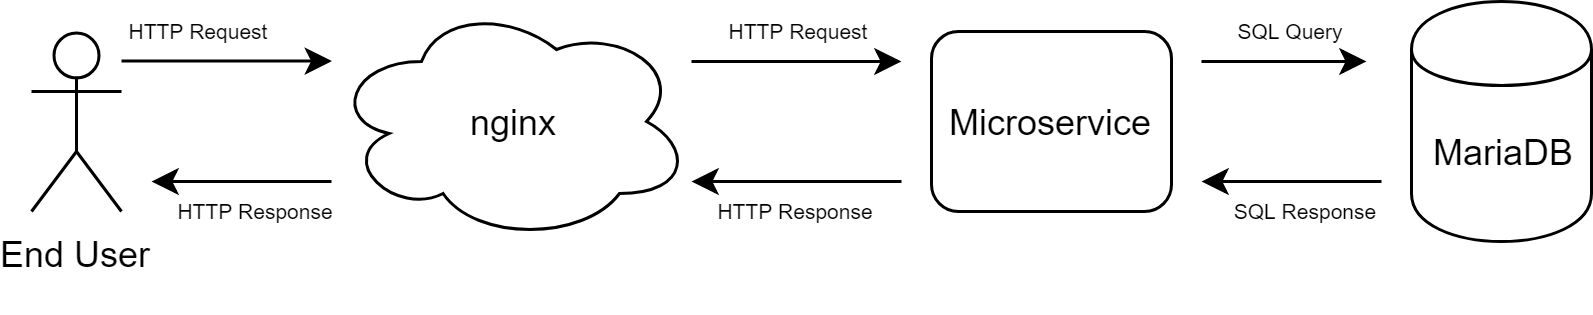
\includegraphics[width=\textwidth]{Images/nginx_proxy_flow.png}
        \caption{Traffic flow diagram showing an end user's browser connecting to the internet facing \textit{nginx} server, which then proxies requests through to the backend microservice}
    \end{figure}
    
    The Aber Fitness system architecture means that not exposed to the internet, but are instead available over an internal Docker network which allows containers to communicate with each other. In order to provide external access to the web servers of all of our microservices we have deployed nginx, an open-source and free web server which features highly customisable config files. Through the use of nginx's \lstinline{proxy\_pass} directive, we are able to take requests from end users and pass them through to the correct backend microservice based on the requested URI. \textbf{TODO: link figure above}
    


\chapter{Implementation}

\section{Deployment}

\section{Java EE}
    \subsection{Common Components}
        \subsubsection{Handling Dependencies and Static Analysis}
        \par
        At the start of the project the JavaEE development teams agreed to use \textit{Maven}\cite{Maven} to handle their dependencies. This allows the entire build process to be ran at the commandline rather than within the IDE, which is essential for \textit{TravisCI} integration.

        \par
        Maven uses an XML file called \textit{POM.xml} to define the dependency names, versions and additional options. These are fetched from Maven Central and cached locally for future builds. To add a new dependency a developer simply visits the hosting website and copies the XML provided alongside each package. Additionally developers can use the \textit{Scope} option which instructs the packaging plugin the associated \textit{JAR} files are provided by the Payara runtime.
        
        \par
        \textit{IntelliJ} natively supports reading from Maven's \textit{POM.xml} file, which defines the list of dependencies and compilation steps. Maven also contains a plugin which allows developers to package the built files into a web archive (WAR). This did have some caveats however; running 
        `\textit{mvn war:war}' would result packaging artefacts from the previous compilation, without compiling the current application. This could lead to confusion as new changes would no be reflected without `\textit{mvn compile war:war}'.

        \par
        Whilst working locally developers could still rely on IntelliJ's built in mechanism for packaging and deploying to a local Payara instance. This allowed for rapid development feedback and iteration without the overhead imposed by Maven.

        \subsubsection{Creating Docker Images}
        \par
        By utilising the ability to run the entire build process on the command-line with Maven we were able to quickly add Travis CI integration. This would clean compile the entire application, run the full \textit{JUnit} test suite and lastly package a WAR file.

        \par
        Initially we used \textit{CheckStyle} to also enforce coding style conventions. However the rules were over-specified. Additionally, unlike other formatting tools there was no option to emit a patch-file which allows developers to automatically fix-up many errors such as incorrect white space or formatting.

        \par
        The Java teams migrated to the \textit{PMD}\cite{PMD} static analysis tool: this warns about unused fields and variables, unsafe constructs,and dangerous coding patterns.
        The Maven test target was modified to run the \textit{PMD}\cite{PMD} static analysis tool before any unit tests. If any violations were detected the build would immediately stop, ensuring all modifications were inspected.

        \par
        The groups proceeded to add a \textit{Dockerfile} to build a docker image for later deployment. Payara provide multiple images on \textit{DockerHub}\cite{DockerHub_Payara}, which range from the full server to an embedded instance.

        \par
        Initially we copied the local web archive, which was built on Travis, into the full Payara deployment folder. This allowed us to use the web administration console to resolve various deployment issues without having to dig through log files. After moving changing the default source code layout, which resolved \textit{resources} not being included in the final archive, we successfully deployed GLaDOS to the full instance.

        \par
        However we could not get Fitbit Ingest to successfully deploy, they had already started implementing the OAuth flow which is required by both the Fitbit API and our own internal API. The internal SSL implementation had changed with JDK update 191, which prevented the \textit{CDI} layer from initialising the associated beans.

        \par
        As the bundled JDK version is controlled by Payara in the base image we proceeded to look for an alternative solution. We decided against modifying the image to transplant a specific JDK at build time. Instead, we found that there was an open upstream issue\cite{payara_ssl_issue} that used reflection to resolve the problem internally. As this fix was not released into the latest stable release we had to switch to running pre-release images for all Java EE applications.

        \subsubsection{Migrating to Micro Image}
        \par
        The Payara Microprofile image is designed specifically to be used in Docker deployments. Whilst this does not implement the full EE, the memory usage is ten times lower at 90MB. The profile still provided the required set of services for the application so there was a significant benefit to completing this migration. However trying to deploy to the micro instance resulted in an exception being thrown whilst completing the implicit bean discovery phase. 

        \par
        The CDI 1.1 specification and above requires the server to automatically scan for injection points and pair it with matching enterprise Java beans (EJBs). This can fail with older dependencies, so we initially suspected one of the dependencies did not correctly use the \textit{beans.xml} annotation to turn this off.
        \newline
        Switching off bean discovery and manually annotating them allowed the ingest service to correctly deploy. However bean discovery is required for Facelets 4.0 and an exception will be thrown if it is not enabled. A new project was created with all but the essential dependencies removed, and we discovered the exception was still thrown which only added to the confusion. 
        
        \par
        By looking at the package namespaces associated with the injection points and running `mvn dependency:tree' we could see that `\textit{org.sonatype.guice}' was the culprit. Walking up the tree we discovered that the WAR plugin was being included in our packaged dependencies. At deployment the microprofile server tried to start a Maven instance and failed, thus removing this dependency correctly allowed the application to start. The development teams realised that the plugin was included in our installed copies so we could still continue to use it.

        \label{JTA_Targets}
        \subsubsection{Setting up JTA Targets}
        Both services started off by instantiating the single JDBC connection through the driver manager as required. This had some caveats however: Firstly, the JDBC driver had to be distributed and managed within the web archive. Secondly, there was no form of connection pooling to allow for scaling at the persistence layer.

        \par
        Traditionally a connection pool is created using the administration web GUI. However this would require a developer set up the pool each time continuous deployment finished on a full instance. The microprofile we had just switched to did not provide a web GUI at all.

        \par
        Glassfish allows a web application to specify resources found on the server using `glassfish-resources.xml'. This XML file can also use system environment variables allowing us to protect and specify database credentials on the deployment targets. The examples found online primarily pertained to a \textit{MySQL} deployment, so multiple iterations of testing and deployment were required to get the pool working successfully. This switch allows an application to detect and create connection pools at deployment, allowing the images to rapidly redeploy facing another database instance.

    \subsection{Fitbit Ingest Service}
        \subsubsection{To Do}

    \subsection{GLaDOS}
        \subsubsection{REST API}
        \par
        The primary role of GLaDOS is to store audit data so that users can view how their data was viewed and modified. Whilst there are native implementations, such as the Java Messaging Service, these require the calls be proxied into a local JVM instance to handle the transport component. We chose to serialise into JSON and use REST as the transport mechanism as all applications had native support for this set up.

        \par
        \textit{JAX-RS} is an API specification for JSON parsing in Java, additionally Payara provides \textit{Jersey} as the implementation of this API at runtime. This avoided us having to package additional dependencies into the web archive. This also allows us to build standard response pages based on the error code internally generated, avoiding having to develop error views.        

        \subsubsection{Unit Testing and Mocks}
        \par
        A new class abstracting the database layer allowed us to avoid writing entity handling at this. We instead focused on writing unit tests which verified the various endpoints correctly serialised or de-serialised data. \textit{Mockito}\cite{Mockito} allows developers to inject mock objects by specifying the class which the test fixture is using.

        \par
        We could not use dependency injection within the endpoint implementation, as the instantiation point is internal to the framework. This doesn't prevent us from using mocks as Mockito allows a developer to inject them through the reflection methods built into the library. A database call such as `\textit{db.getEntry(id)}' could be tested to see which status codes would be sent and verify the data,if any, was serialised correctly.

        \subsubsection{Integration Testing with Arquillian}
        \textit{Arquillian}\cite{Arquillian} allows developers to specify the classes to archive and deploy within the text fixture. Payara also provides an embedded Arquillian test container which can be ran at test time to exercise sections of a full system. This would allow us to write integration tests for an end-to-end operations, such as POSTing data to an endpoint and ensuring it is written to the persistence layer.

        \par
        There was extensive documentation on the methods required to pack an archive, but limited examples on handling Maven dependencies. As the embedded instance provides no runtime methods we were having problems getting the container to correctly run. Developers could specify the full class paths for their dependencies to ensure the were packaged, but this was extremely verbose and fragile.

        \par
        We looked into using the Maven dependency resolver, which allows developers to get a list of runtime Jars and package them into the archive. However this would led to another set of problems where Maven was trying to export them into a \textit{.zip} format, then throw an exception because this was not supported.

        \par
        With no easy was to control the format that runtime dependencies were exported in, combined with a lack of documentation pertaining specifically to Maven we agreed to abandon this method of automated testing. This would give us more time for implementing other components within the deadline. We opted to rely on manual integration testing for the duration of the project instead.

        \subsubsection{Entity Management}
        This service only persists Audit Data, therefore we ultimately need to persist a single entity. Whilst many ORM solutions exists for Java, such as \textit{Hibernate}, we decided against them due to the implementation overhead that was required.

        \par
        Instead we relied on the persistence layer provided in the EE specification. Using the connection pools which were set up for both Java services (see \ref{JTA_Targets}), we could specify which JTA the injected entity manager should use.

        \par
        The table schema is managed through annotations on an entity class. This also allows the implementation provided by Payara, \textit{EclipseLink}, to create the tables required at deployment time. As the framework relies on the field types to determine which underlying storage to use there is a hidden pitfall. If the type does not have a native serialisation Java will try to persist this using binary data.

        \par
        Instants are used to specify timestamps on logs, these are cross compatible as they use \textit{ISO 8601}\cite{ISO_8601}, a string specifier for absolute time points. This format allows both .NET Core and Java application to send timestamps in the following format \textit{2018-11-28T12:04:14Z}. However as this type was added in JDK 8 there is no native storage conversion built into the entity framework.

        \par
        Two adaptors were written based on the \textit{AttributeConverter} interface. These provide methods for marshalling and un-marshalling Instants into String objects, which the entity manager can easily store. Annotating the field installed the converting class and correctly updated the schema. This also has the added benefit of making the stored timestamps human readable within the database, which extremely helpful for debugging.

        \subsubsection{Developing Facelets}
        \par
        GLaDOS also provides a page that allows a user to retrieve audit data associated with their account. Administrators can look up any users audit data by user their unique ID too. In addition there is a status page which allows anyone to view the status of all other micro-services without logging in.

        \par
        The front-end of GLaDOS use facelets to implement the MVC pattern. A backing bean for the user data uses named queries from the persistence layer to retrieve data into a list of entity objects. We switched to using \textit{PrimeFaces}\cite{Primefaces}, which is a fork of the now deprecated \textit{RichFaces}. This allows us to use components such as \textit{DataTables} which dynamically generate tables based on the number of entries returned.

        \par
        The Fitbit Ingest Service had completed OAuth implementation for connecting to internal and external APIs. This was ported across to GLaDOS and further modified. As the ingest service has no front-end they don't need to persist \textit{JSON Web Tokens (JWTs)}. Additional methods were written specifically for this microservice. These include using the HTTP session handling built into the web framework to persist the token on the server. Another helper class was written which validates the stored JWT as the user navigates through protected pages, or POSTs any requests.

        \par
        Service statuses were implemented using a singleton Java bean which is instantiated at deployment. Using the scheduling capability provided for EJBs we poll all services every 20 seconds in a seperate thread. All services implement an endpoint at \textit{/api/status} that returns a 200 or 204. This is stored until the page is retrieved where the backing bean, acting as a presenter forward the results on.

        \par
        As the application stack uses an \textit{nginx} instance to reverse proxy queries the URLs must take this into account when they are generated within the facelet. .NET Core makes this trivial by calling `\textit{App.UsePathBase(URL)}' at start up, however Java applications rely on the context root. This was interfering with the URL rewriting that Nginx performs resulting in the service using the 
        `\textit{/glados/glados/}' base path.

        \par
        Initially we used an environment variable to manually generate links between the pages of the service and set the context root to 
        `\textit{/}'. However, this quickly proved to be untenable when using forms, as POST requests were being sent to 
        `\textit{/destination}' 
        rather than 
        `\textit{/glados/destination}'. Ultimately to work around this an exception was added to Nginx configuration to avoid re-writing any URLs for GLaDOS, and instead rely on the service to correctly address all requests. This allowed us to switch back to generating addresses based on the \textit{outcome} tag and use forms on the service.



\section{.NET Core}
    \subsection{}{Common Components}
some blurb about .net core here

    \subsection{Booking Facilities}

    \subsection{Challenges}

    \subsection{Communications}

    \subsection{Gatekeeper}

    \subsection{Health Data Repository}

    \subsection{Health Dashboard}

    \subsection{Ladders}

    \subsection{User Groups}

\chapter{Testing}
\par
One of the core tenets of continuous deployment is the reliance on a mix of automated and manual testing to ensure a system is functioning correctly. The applicable subset of these tests were run before each change specified in a pull request was accepted. The full suite was run as part of the release process, which allowed developers to deploy the application to production with confidence.

\section{Unit Testing}
\par

\par
\subsection{Framework Choices}
\textit{.NET Core} and \textit{Java EE} both have a host of unit testing frameworks to choose from. In order to maintain consistency, it was decided that the a single framework would be used for all \textit{.NET Core} applications and another single framework for every \textit{Java EE} application. The development teams agreed on using \textit{xUnit}\cite{xUnit} for .NET Core, and \textit{JUnit}\cite{JUnit} for \textit{Java EE} early into the project.

\par
For \textit{.NET Core} applications, xUnit was chosen in place of \textit{MSTest} and \textit{NUnit}. Recent documentation and examples from Microsoft have focused on xUnit instead of MSTest. xUnit is significantly more extensible through the use of the \textit{Theory} attribute, allowing a single test method to be written for multiple datasets.

\par
Additionally, xUnit extends upon principles found in NUnit with additional features, such as the ability to execute individual test methods\cite{Nunit_XUnit_comparison}. It also instantiates a new test instance for each fixture, ensuring that side effects do not propagate through a test suite. This prevents problems with ordering tests found in some software projects.

\par
JUnit is an almost ubiquitous testing framework for \textit{Java EE} for a few reasons; it has strong integration with other tools, such as Maven and various mocking frameworks, and documentation is widely available. Multiple versions exist so the \textit{Java EE} teams chose to use version 5, as it is the latest stable release on JUnit.

\subsection{Mocking}
\par
\textit{Moq}\cite{Moq} is used for mocking injected dependencies in \textit{.NET Core} services. Classes were written using the dependency injection pattern, accepting a concrete type at construction time. Using Moq objects is extremely simple; developers instantiate their mock based on an interface, then set up expectations, if any, and verify the calls.  The library also allows developers to provide mock implementations of methods available on the interface to enable more in-depth testing of the component.

\par
\textit{Java EE} requires a slightly different approach, as an EJB cannot have arguments in its constructor. \textit{Mockito}\cite{Mockito} provides an alternative to dependency injection; developers create fields in the class which match the types which are constructed in the EJB. These are annotated with `\textit{@mock}' and subsequently injected with `\textit{@injectMocks}' on the test instance. Mockito supports \textit{Hamcrest}\cite{Hamcrest} matchers which were also used to handle more complex assertions.


\section{Integration Testing}
\par
Most of the micro-services provide internal APIs, which are not designed for external usage. To protect these endpoints the OAuth 2.0 flow was used to authorize application interactions with client credentials. Whilst unit testing ensures each API correctly responds according to its documented behaviour, it does not exercise all components that partake in an interaction.

\par
As REST endpoints were used as the primary message exchange method we could send and request JSON payloads to ensure the system under test behaved as expected. Multiple third party solutions were used for testing APIs, \textit{Postman}\cite{Postman} was one instance that was widely used by the development team. 
This can handle the OAuth flow 

\par
Developers used these tools to ensure that malformed requests or interaction with no authorization token were correctly handled. Additionally they can handle the OAuth flow on a developers behalf, this was extremely useful when debugging interactions between applications and resolving digressions from the API specifications.


\section{System Testing}
\par
Aber Fitness was deployed onto two separate \textit{Docker} hosts, representing staging and production. Developers could trigger a deployment from the latest development images in \textit{Slack}, and then manually test the system in a deployed state. This also allowed for the detection of deployment specific problems, which are un-testable without a complete system.

\par
One example of an issue caught by manual system testing was within the \textit{Challenges} microservices, which contained a controller which was not operating asynchronously. Unit tests would not exercise the instance in parallel, so this bug was not caught in unit testing. The bug resulted in API calls made to the deployed application returning a HTTP 502 response, due to the original call putting the controller in a blocked state and preventing it from responding to the next call.


\section{Static Analysis}
\subsection{PMD}
\par
Initially, Java used \textit{CheckStyle} to also enforce coding style conventions. However, the rules were far too strict to be beneficial or practical and, unlike other formatting tools, there was no option to emit a patch-file which allows developers to automatically fix-up many errors such as incorrect white space or formatting.

\par
The Java teams later migrated to the \textit{PMD}\cite{PMD} static analysis tool: this warns about unused fields and variables, unsafe constructs, and dangerous coding patterns.
The Maven test target was modified to run the PMD static analysis tool before any unit tests. If any violations were detected the build would immediately stop, ensuring all modifications were inspected.

\section{Acceptance Testing}
\par
During our first meeting, the project's functional requirements were broken down into a number of spreadsheets, each based on the service which would implement them. The client was then contacted to clarify any requirements which were ambiguous to the group. Acceptance tests for each micro-service were added to a spreadsheet based on these original and revised requirements.

\par
Acceptance tests are completed manually by completing the steps defined by the document. Each test is marked as pass or fail based on the criteria also set out in the document, allowing the individual microservices, and by extension the entire project, to be assessed on its fitness for purpose.

\par
A fresh deployment of the system was performed shortly after a code freeze and the full suite of acceptance tests were completed. This round of testing highlighted 23 instances where the implementation deviated from the client's requirements.

\par
Bugs were assessed on a case-by-case basis, taking account of the impact. Fixes which had a low potential for regression and addressed high impact problems were implemented and merged after the code freeze. This process resolved 11 of those implementation issues, resulting in almost half of the failed acceptance tests becoming passes in the space of a few hours, and with no additional issues appearing as side-effects. This shows that internal acceptance testing was a highly valuable process that resulted in a noticable improvement in the final product.


\chapter{Status}
\chapter{Evaluation}

\section{Development Methodology}

  \subsection{Evaluation}
  \par
  The group met for weekly meetings at the start of the project to define a top-level system design on a whiteboard. These sessions were initially productive, as work was distributed to subteams and a unified approach for the various microservices was decided. As the project went on, the usefulness of these meetings was questioned. Attempts to design by committee would rapidly devolve into either a few interested parties talking about a single service, or every developer inputting an opinion on simple decisions.

  \par
  A vote unanimously agreed to change the group meeting into a session where every developer would work on implementation in the same room instead. This refocused teams onto their own design, whilst allowing an individual to still propose system-level questions or ideas in person. Productivity also rapidly increased as knowledge of common problems and solutions were shared amongst the group.

  \par
  Throughout the project there have been instances where the requirements were not clear. Reasons ranged from multiple interpretations, noun and verb conflation, and insufficient detail. Slack was used as a communication mechanism with the client, which allowed the client to choose an appropriate time to respond to requests, which could be sent at any time, while also enabling real time discussion. These communications taking place over a recorded medium meant that an answer could easily be converted into an additional requirement later.

  \par
  As the project progressed, Scrumban-related processes were skipped increasingly. Project boards weren't being updated or tracked and work was completed without an associated issue or project board entry. As there were eight members of the group, it became increasingly difficult to track the work that individual teams had remaining. Ultimately this lead to deadlines being missed, as teams had to estimate their work left to complete rather than having a metric to rely on.

  \par
  As the scope of each unit's work was not defined, branches would often contain multiple features and fixes. Pull requests would often alternate between being too large to sensibly review, or a single fix spread across several pull requests. Additionally, developers would typically review within a subteam, instead of examining other services' code. This lead to code reviews being approved without the approver properly reviewing the change. This culminated into several simple bugs and version control issues, which would likely have been spotted, such as incorrect equality comparisons being merged into the codebase.


\section{Future Improvements}

- \\TODO Blocked on status

- Integration Testing

\section{Fitness for purpose}
    \subsection{Functional Requirements}
    \par
    Based on the client's criteria we have fulfilled the majority of functional requirements, as seen in \ref{Requirements_chpt}. This was measured using acceptance tests which give a rough indication of conformity to the requirements. \\TODO tests were performed with \\TODO failing, giving a \\TODO \% final pass rate.

    \subsection{Design Constraints}
    \par
    Our application stack makes use of both Java EE and .NET Core, as per the design constrains. These languages also provide access to many frameworks and third party implementation through Nuget and Maven. 
    
    \par
    By carefully checking the license of all external code and finding alternatives where required, the system is completely free of proprietary software and licensing considerations. Additionally, this reliance on external packages for core components,such as \textit{Identity Server} for authorization, reduces the sites future maintenance overhead.

    Finally, deployable docker images were created for each microservice which ran on the destination server. This would also allow the system to scale the number of instances based on an individual service's load in the future.

% add any additional chapters here

\setemptyheader
\addcontentsline{toc}{chapter}{Appendices}
\chapter*{Appendices}

\pagebreak

% start the appendix - sets up different numbering
\fancypagestyle{plain}{%
%\fancyhf{} % clear all header and footer fields
\fancyhead[L]{\textsl{Appendix\ \thechapter}}
\fancyhead[R]{\textsl{\leftmark}}}

\appendix
\fancyhead[L]{\textsl{Appendix\ \thechapter}}
\fancyhead[R]{\textsl{\leftmark}}
\fancyhead[C]{}
\fancyfoot[C]{\thepage}
\renewcommand{\headrulewidth}{0.4pt}
\renewcommand{\chaptermark}[1]{\markboth{#1}{}}

\fancyhead[L]{\textsl{Appendix\ \thechapter}}
\fancyhead[R]{\textsl{\leftmark}}
\fancyfoot[C]{{\thepage} of \pageref{LastPage}}



% include any appendices here
\bibitem{SignalR} "Introduction to ASP.NET Core SignalR" Available at: https://docs.microsoft.com/en-us/aspnet/core/signalr/introduction?view=aspnetcore-2.2 [Accessed: 16- Dec- 2018]

\section{Appendix 2 - Acceptance Testing}

\subsection{Site Wide}
	\begin{longtable}{ |l|p{3cm}|l|p{5cm}|p{5cm}|l|p{6.5cm}|}
\hline
\textbf{FR\#}	&	\textbf{Requirement} & \textbf{AT\#}	&	\textbf{Description} & \textbf{Test} & \textbf{Pass/Fail} &	\textbf{Comments} \\
\hline
\endhead

&  & S-AT-1 & The webpages should display who is currently logged in, & In the top corner of the webpages "Logged in as" should be displayed followed by the username/userid & Pass &  \\ \hline
 &  & S-AT-2 & If a user is not logged in and try to access a page, they will be redirected to the login form. & No user logged in. Try to access booking facilities. Will be required to login. & Pass &  \\ \hline
EIR-1 & The system should be a set of microservices and accessible from a web browser & S-AT-3 & Check the website is accessible from a browser & Navigate to the Aber Fitness website using a browser & Pass &  \\ \hline
EIR-2 & The system should support localisation without having to provide translations & S-AT-4 & Check the website supports localisation & Switch the browser's preferred language to something else, e.g. Welsh. Check some sample translations are loaded & Fail & The system does not support localisation. \\ \hline
 &  & S-AT-5 &  &  &  &  \\ \hline

\end{longtable}


\subsection{Booking \& Facilities}
	\begin{longtable}{ |l|p{3cm}|l|p{5cm}|p{5cm}|l|p{6.5cm}|}
\hline
\textbf{FR\#}	&	\textbf{Requirement} & \textbf{AT\#}	&	\textbf{Description} & \textbf{Test} & \textbf{Pass/Fail} &	\textbf{Comments} \\
\hline
\endhead


BS-FR1-1 & Facilities - manage venues/facilities/sports link & BS-AT-1 & As an admin - a link will be available on the bookings webpage to manage facilities, sports and venues. When this is pressed the admin will be redirected to the facilities management webpage. & When an admin presses the "manage facilities/venues/sports" link, brings up the management page. & Pass & \\
\hline

BS-FR1-1 & Facilities - manage facilities & BS-AT-2 & As an admin - once redirected to the management page, a list of facilities will be available (can be empty) & A list of facilities should be present. This list can be empty if no facilities have been entered, this may be blank. & Pass & \\
\hline

BS-FR1-1 & Facilities - manage venues link & BS-AT-3 & As an admin - A link will be available on the facilities and sports webpages to redirect the admin to the manage venues page.  & When the link is clicked by the admin, it should bring up the venues page. & Pass & \\
\hline

BS-FR1-1 & Facilities - manage sports link & BS-AT-4 & As an admin - A link will be available on the venues and facilities webpages to redirect the admin to the manage sports page.  & When the link is clicked by the admin, it should bring up the sports page. & Pass & \\
\hline

BS-FR1-1 & Facilities - manage facilities link & BS-AT-5 & As an admin - A link will be available on the venues and sports webpages to redirect the admin to the manage facilities page.  & When the link is clicked by the admin, it should bring up the facilities page. & Pass & \\
\hline

BS-FR1-1 & Facilities - add venue link & BS-AT-6 & As an admin - when viewing the list, an add venue link will be available. When this is pressed the admin will be redirected to the add venue webpage. & When viewing the list of venues, click the add button. This should redirect the admin to an add venue page. & Pass & \\
\hline

BS-FR1-1 & Facilities - add venue & BS-AT-7 & As an admin - The add venue webpage will contain a form. This form will enable the user to add a venue name e.g. Old Sports Hall. Once this has been entered, the confirm button can be pressed and, if the venue name doesn\'t already exist, the new venue should be added. If the venue name already exists, the user will be alerted. If the user clicks cancel nothing will change. & 1. User enters name that already exists. Click Confirm. User will be alerted (nothing will change). 2. User adds name. Click Cancel (nothing will change). 3. User enters name that doesn\'t exist. Click Confirm. Venue will be added. & Pass & \\
\hline

BS-FR1-1 & Facilities - remove venue & BS-AT-8 & As an admin - when viewing the list of venues, a remove venue link will be available. Pressing this will alert the user that they are about to remove the venue and all facilities linked to said venue. If the user clicks confirm then the venue will be removed. If the user clicks cancel, nothing will change. & 1. User clicks remove venue. Click Cancel (nothing will change). 2. User clicks remove venue. Click Confirm. Venue and linked facilities should be removed. & Pass & \\
\hline

BS-FR1-1 & Facilities - update venue link & BS-AT-9 & As an admin - when viewing the list, an update venue link will be available for each venue. When this is pressed the admin will be redirected to the update venue webpage for that venue. & When viewing the list of venues, click the update button. This should redirect the admin to an update venue page. & Pass & \\
\hline

BS-FR1-1 & Facilities - update venue & BS-AT-10 & As an admin - The update venue webpage will contain a form. This form will enable the user to change the venue name e.g. New Sports Hall. Once this has been entered, the confirm button can be pressed and, if the venue name doesn\'t already exist, the updated venue should be stored. If the venue name already exists, the user will be alerted. If the user clicks cancel nothing will change. & 1. User clicks update venue. User changes name to name that already exists. Click Confirm. User will be alerted (nothing will change). 2. User clicks update venue. User changes name. Click Cancel (nothing will change). 3. User clicks update venue. User changes name to that doesn\'t exist. Click Confirm. Venue name will be changed. & Pass & \\
\hline

BS-FR1-1 & Facilities - add facility link & BS-AT-11 & As an admin - when viewing the list, an add facility link will be available. When this is pressed the admin will be redirected to the add facility webpage. & When viewing the list of venues, click the add button. This should redirect the admin to an add venue page. & Pass & \\
\hline

BS-FR1-1 & Facilities - add facility & BS-AT-12 & As an admin - The add facility webpage will contain a form. This form will require the selection of a venue (e.g. Old Sports Hall), a facility name (e.g. Court 1) and a list of sports that can be played (e.g. squash, tennis). Once this has been entered, the confirm button can be pressed and, if the facility name doesn\'t already exist for this venue, the new venue should be added. If the facility name already exists for this venue, the user will be alerted. If the user clicks cancel nothing will change. & 1. User enters name that already exists in facilities. Click Confirm. User will be alerted (nothing will change). 2. User adds name. Click Cancel (nothing will change). 3. User enters name that doesn\'t exist in venue. Click Confirm. Facility will be added. & Pass & \\
\hline

BS-FR1-1 & Facilities - remove facility & BS-AT-13 & As an admin - when viewing the list of facilities, a remove facility link will be available. Pressing this will alert the user that they are about to remove the facility. If the user clicks confirm then the facility will be removed. If the user clicks cancel, nothing will change. & 1. User clicks remove facility. Click Cancel (nothing will change). 2. User clicks remove facility. Click Confirm. Facility should be removed. & Pass & \\
\hline

BS-FR1-1 & Facilities - update facility link & BS-AT-14 & As an admin - when viewing the list, an update facility link will be available for each facility. When this is pressed the admin will be redirected to the update facility webpage for that facility. & When viewing the list of facilities, click the update button. This should redirect the admin to an update facility page. & Pass & \\
\hline

BS-FR1-1 & Facilities - update facility & BS-AT-15 & As an admin - The update facility webpage will contain a form. This form will enable the user to change the facility name e.g. Court 2. Once this has been entered, the confirm button can be pressed and, if the facility name doesn\'t already exist for this venue, the updated facility should be stored. If the facility name already exists for this venue, the user will be alerted. If the user clicks cancel nothing will change. & 1. User clicks update facility. User changes name to name that already exists for venue. Click Confirm. User will be alerted (nothing will change). 2. User clicks update facility. User changes name. Click Cancel (nothing will change). 3. User clicks update facility. User changes name to that doesn\'t exist. Click Confirm. Facility name will be changed. & Pass & \\
\hline

BS-FR1-1 & Facilities - add sport link & BS-AT-16 & As an admin - when viewing the list, an add sport link will be available. When this is pressed the admin will be redirected to the add sport webpage. & When viewing the list of sports, click the add button. This should redirect the admin to an add sport page. & Pass & \\
\hline

BS-FR1-1 & Facilities - add sport  & BS-AT-17 & As an admin - The add sport webpage will contain a form. This form will enable the user to add a sport name e.g. Squash. Once this has been entered, the confirm button can be pressed and, if the sport name doesn\'t already exist, the new sport should be added. If the sport name already exists, the user will be alerted. If the user clicks cancel nothing will change. & 1. User enters name that already exists. Click Confirm. User will be alerted (nothing will change). 2. User adds name. Click Cancel (nothing will change). 3. User enters name that doesn\'t exist. Click Confirm. Sport will be added. & Pass & \\
\hline

BS-FR1-1 & Facilities - remove sport & BS-AT-18 & As an admin - when viewing the list of sports, a remove sport link will be available. Pressing this will alert the user that they are about to remove the sport and all facilities with only this sport assigned to them. If the user clicks confirm then the sport and all stipulated facilities will be removed. If the user clicks cancel, nothing will change. & 1. User clicks remove sport. Click Cancel (nothing will change). 2. User clicks remove sport. Click Confirm. Sport and linked facilities should be removed. & Pass & \\
\hline

BS-FR1-1 & Facilities - update sport link & BS-AT-19 & As an admin - when viewing the list, an update sport link will be available for each sport. When this is pressed the admin will be redirected to the update sport webpage for that sport. & When viewing the list of sport, click the update button. This should redirect the admin to an update sport page. & Pass & \\
\hline

BS-FR1-1 & Facilities - update sport & BS-AT-20 & As an admin - The update sport webpage will contain a form. This form will enable the user to change the sport name e.g. Tennis. Once this has been entered, the confirm button can be pressed and, if the sport name doesn\'t already exist, the updated sport should be stored. If the sport name already exists, the user will be alerted. If the user clicks cancel nothing will change. & 1. User clicks update sport. User changes name to name that already exists. Click Confirm. User will be alerted (nothing will change). 2. User clicks update sport. User changes name. Click Cancel (nothing will change). 3. User clicks update sport. User changes name to that doesn\'t exist. Click Confirm. Sport name will be changed. & Pass & \\
\hline

BS-FR2-1 & Availability - link & BS-AT-21 & As an admin - on the home page there will be a link that says"Block facility" This will allow the admin to book a facility for a period of time. Clicking this link will redirect the admin to a period booking webpage. & When viewing the list of facilities, click the book period button. This should redirect the admin to a book period page. & Pass & \\
\hline

BS-FR2-1 & Availability - Book period & BS-AT-22 & As an admin - on the book period page for a facility, the admin has the ability to choose a start and end date as well as input a reason for the booking. The admin can confirm the booking, or cancel the action. Confirming will book the facility for that duration of time.  & 1. Click cancel, page will go back and nothing will change. 2. Input valid information into the form. The facility will no longer be available for that period. & Pass & \\
\hline

BS-FR3-1 & Booking - view bookings & BS-AT-23 & As a member - you can view your bookings. This will be displayed as a list. If no bookings have been made then only blocked facilities will be shown. & A list of member bookings should be present. This list can be empty if no booking\'s have been entered, this may be blank. & Pass & \\
\hline

DG-FR9-1 & Booking - view bookings (admin) & BS-AT-24 & As an admin - you can view all bookings made by members. This will be displayed as a list. If no bookings have been made then this will be empty. & A list of member bookings should be present. This list can be empty if no booking\'s have been entered, this may be blank. & Pass & \\
\hline

BS-FR3-1 & Booking - add booking link & BS-AT-25 & As a member - when viewing the list, an add booking link will be available. When this is pressed the member will be redirected to the add booking webpage. & When a member is viewing their bookings, click the add button. This should redirect the member to an add booking page. & Pass & \\
\hline

BS-FR3-1 & Booking - add booking (choose date, sport and venue) & BS-AT-26 & As a member - once being redirected to the add bookings page, member will be able to fill in the form by selecting venue, sport and date for the booking. Clicking cancel will redirect the member back to the previous page. Clicking confirm will redirect the member to the choose time page. If no times are available for the day the member will be alerted. & 1. User fills in form data. Click Cancel (nothing will change). 2. User fills in form data. Click confirm. User will be directed to choose a time. 3. If no times for the date are available the user should be alerted that no times are available. & Pass & \\
\hline

BS-FR3-1 & Booking - add booking (choose time) & BS-AT-27 & As a member - user will be presented with list of a times for the specified date. User can select one of these times. If user presses cancel, they will be redirected to the previous page (add bookings). If user presses confirm, they will receive a message confirming their booking and a court. & 1. User selects time. User presses cancel, redirected to add bookings page. 2. User selects time. User presses confirm, receive confirmation of time and an assigned court. & Pass & \\
\hline

BS-FR3-1 DG-FR9-1 & Booking - remove booking & BS-AT-28 & As an member and admin - when viewing the list of bookings, a remove booking link will be available. Pressing this will alert the user that they are about to remove the booking. If the user clicks confirm then the booking will be removed and the time will become available . If the user clicks cancel, nothing will change. & 1. User clicks remove booking. Click Cancel (nothing will change). 2. User clicks remove booking. Click Confirm. Booking should be removed and time should be freed. & Pass & \\
\hline

BS-FR3-1 DG-FR9-1 & Booking - update booking link & BS-AT-29 & As a member and admin - when viewing the list, an update booking link will be available. When this is pressed the user will be redirected to the update booking webpage. & When viewing the list of bookings, click the update button. This should redirect the user to an update sport page. & Pass & \\
\hline

BS-FR3-1 DG-FR9-1 & Booking - update booking (choose date, sport and venue) & BS-AT-30 & As a member and admin - once being redirected to the update bookings page, user will be able to update the form data by selecting a venue, sport and date for the booking. Clicking cancel will redirect the user back to the previous page. Clicking confirm will redirect the user to the choose time page. If no times are available for the day the user will be alerted.  & 1. User Clicks Cancel (nothing will change). 2. User updates form data. Click confirm. User will be directed to choose a time. 3. If no times for the date are available the user should be alerted that no times are available. & Pass & \\
\hline

BS-FR3-1 DG-FR9-1 & Booking - update booking (choose time) & BS-AT-31 & As a member and admin - user will be presented with a list of a times for the specified date. User can select one of these times. If user presses cancel, they will be redirected to the previous page (add bookings). If user presses confirm, they will receive a message confirming their booking has changed, and confirming a court. Booking\'s original time will then be freed up. & 1. User selects time. 2. User presses cancel, redirected to add bookings page. 3. User presses confirm, receives confirmation of time and an assigned court (booking in old timeslot is removed). & Pass & \\
\hline

BS-FR4-1 & Booking - 1 hour time slot & BS-AT-32 & As a member - When bookings are being made they should be in hour time slots. & Click add booking. Enter date, venue and sport. Click confirm. The dates returned should be 1 hour time slots.  & Pass & \\
\hline
\end{longtable}

\subsection{Challenges}
	\subsubsection{Overall Functionality}
\par
The \textit{Challenges} microservice was created to set personal and group challenges. When creating a challenge, a member has the ability to select an activity, goal metric and goal within a time frame. The group challenges are specific to a single group, and can only be joined by users within that group. \textit{Challenges} is the only microservice to use the coordinator user type, with coordinators being able to create group challenges. 

\subsubsection{MVC Architecture}
\par
As the microservice requires CRUD operations on data, it was essential that a persistence layer was present.
Initially the microservice consisted of \textit{Challenge} and \textit{Activity} model-view-controllers, but this proved to be inadequate when it came to database normalisation. The architecture underwent many alterations, eventually resulting in \textit{UserChallenge}, \textit{ChallengeManage}, \textit{Activity} and \textit{GoalMetric} as the final model-view-controllers, with \textit{ChallengeManage} only named as such due to an issue with \textit{nginx}. The \textit{UserChallengeController} is used to keep track of a user's group and personal challenges.

\par
The index pages for \textit{UserChallenge} and \textit{ChallengeManage} display all of the user's challenge information and group challenges respectively. The \textit{ChallengeManageController} is used to handle all existing challenges. A challenge is assigned both a \textit{GoalMetricId} and an \textit{ActivityId}. The \textit{ActivityController} and \textit{GoalMetricController} allow admins and coordinators to modify activities and goal metrics. The activities are retrieved from the \textit{Health Data Repository} and the goal metrics must be manually entered to match the database key.

\subsubsection{API Access}
\par
The microservice requires access to the \textit{Health Data Repository} to retrieve data in order to update the progress of a challenge. When the user challenges page or API endpoint is accessed, their challenges are updated with the most recent data.
Access is also required to \textit{User Groups} to retrieve information about a user or group. A user will only see challenges for their group on the group challenges page. 
In addition access is required to the \textit{Communications} microservice, in order to send notifications to users when their challenges close.

\subsubsection{API Endpoints}
\par
The \textit{Health Dashboard} requires access to the \textit{Challenges} microservice to display personal and group challenges and create the former. Displaying challenges on the \textit{Health Dashboard} required retrieving a user's personal and group challenges, which necessitated \textit{GET} endpoints. \textit{POST} endpoints were needed to create a challenge and associated user challenge. As the challenge can only be created for specific activities, the \textit{Health Dashboard} must also retrieve a list of available activities from a \textit{GET} endpoint.
Although the functionality was ultimately not implemented, the \textit{PUT} endpoint was created to allow the \textit{Health Dashboard} microservice to update existing personal challenges.
A status endpoint was necessary for \textit{GLaDOS}, so that the current status of the microservice could be displayed.

\subsubsection{User Interface}
\par
As this microservice is responsible for managing user data, the majority of the user interface was generated using scaffolding functionality. Most of the pages were adapted to display the desired contents, depending on the identity of a user.


\subsection{Fitbit Ingest Service}
	\begin{longtable}{ |l|p{3cm}|l|p{5cm}|p{5cm}|l|p{6.5cm}|}
\hline
\textbf{FR\#}	&	\textbf{Requirement} & \textbf{AT\#}	&	\textbf{Description} & \textbf{Test} & \textbf{Pass/Fail} &	\textbf{Comments} \\
\hline
\endhead



\end{longtable}

\subsection{Gatekeeper}
	During the analysis and planning stages it quickly became apparent that a central authentication and authorization system would be required.  The Gatekeeper service is responsible for providing this, and does so by acting as both an OAuth 2.0 Authorization Server, and an OpenID Connect Identity Provider (IDP).  Such a setup provides a number of benefits, including seamless Single Sign-On (SSO), relative ease of implementation due to the abundance of available libraries, separation of concerns by decoupling authentication \& authorization from each microservice, and the theoretical ability to allow third-party access to AberFitness APIs in the future.

\subsubsection{IdentityServer 4}

Rather than attempting to implement our own OAuth 2.0 server, it seemed beneficial in terms of both security and development time to use an existing solution.  After thorough investigation of the available implementations, IdentityServer 4 was chosen as it not only fully implements the specification of OAuth 2.0 and OpenID Connect, but is also certified by the OpenID Foundation, and is part of the .NET Foundation.  Thorough documentation is available, the project is open-source with a permissive license, and the library is specifically designed for .NET Core 2.

\subsubsection{OAuth Overview}

Two basic OAuth 2.0 flows are used within AberFitness - Authorization Code (including the hybryid flow OpenID Connect extension) for applications with a GUI wishing to identify users, and Client Credentials for API authorization between the various microservices.

When a user first attempts to access a service where authentication is required, they are redirected to Gatekeeper in order to log in.  Once logged in, they are redirected back to the client application which completes a token validation process in order to verify the login.  To facilitie SSO, users which are already logged in to Gatekeeper will be seamlessly redirected back to the client application with no action required from them.

[Flow diagram]

On subsequent requests, a redirect to Gatekeeper is not usually required.  Access tokens are valid for one hour, with the client being able to obtain new tokens via the use of a refresh token.  Redirection to Gatekeeper should only be required if the user has cleared their browser cookies, or those cookies have become invalidated for some reason.

[Flow diagram]

When a microservice wishes to call the API of another microservice, they obtain a client credentials access token from Gatekeeper, and send it in the Authorization header of the request they are making.  Access tokens have a limited number of scopes (services) for which they are valid, and the service receiving the request will reject the token should it not contain the scope required for that service.  Once the content of access token has been checked, the signature of the token is validated using the JSON Web Key Set (JWKS) available from Gatekeeper.  This is essentially a public key which can be used to verify that the access token was indeed issued by Gatekeeper.

[Flow diagram]


There was some consideration as to whether client credentials was the correct flow to use for authorization when obtaining user resources within AberFitness.  Typically you would require an access token specific to that user, obtained using the authorization code flow, in order to access resources such as activity data belonging to that user.  Eventually it was decided that the authorization code flow would be more relevant to third-party applications wishing to access our APIs.  As all microservices within AberFitness can be considered as belonging to the same overall system, it seemed that the client credentials flow was sufficient to authorize access to data from other services within the AberFitness system.

\subsubsection{Implementation Details}

client libraries

data protection keys

no editing

schema complexity

\subsubsection{Alternatives}

.NET alternatives

Java implementations

SAML

API gateway


\subsection{GLaDOS}
	\subsubsection{REST API}
\par
The primary role of GLaDOS is to store audit data so that users can view how their data was viewed and modified. Whilst there are native implementations, such as the Java Messaging Service, these require the calls be proxied into a local JVM instance to handle the transport component. We chose to serialise into JSON and use REST as the transport mechanism as all applications had native support for this set up.

\par
\textit{JAX-RS} is an API specification for JSON parsing in Java, additionally Payara provides \textit{Jersey} as the implementation of this API at runtime. This avoided us having to package additional dependencies into the web archive. This also allows us to build standard response pages based on the error code internally generated, avoiding having to develop error views.        

\subsubsection{Unit Testing and Mocks}
\par
A new class abstracting the database layer allowed us to avoid writing entity handling at this. We instead focused on writing unit tests which verified the various endpoints correctly serialised or de-serialised data. \textit{Mockito}\cite{Mockito} allows developers to inject mock objects by specifying the class which the test fixture is using.

\par
We could not use dependency injection within the endpoint implementation, as the instantiation point is internal to the framework. This doesn't prevent us from using mocks as Mockito allows a developer to inject them through the reflection methods built into the library. A database call such as `\textit{db.getEntry(id)}' could be tested to see which status codes would be sent and verify the data,if any, was serialised correctly.

\subsubsection{Integration Testing with Arquillian}
\textit{Arquillian}\cite{Arquillian} allows developers to specify the classes to archive and deploy within the text fixture. Payara also provides an embedded Arquillian test container which can be ran at test time to exercise sections of a full system. This would allow us to write integration tests for an end-to-end operations, such as POSTing data to an endpoint and ensuring it is written to the persistence layer.

\par
There was extensive documentation on the methods required to pack an archive, but limited examples on handling Maven dependencies. As the embedded instance provides no runtime methods we were having problems getting the container to correctly run. Developers could specify the full class paths for their dependencies to ensure the were packaged, but this was extremely verbose and fragile.

\par
We looked into using the Maven dependency resolver, which allows developers to get a list of runtime Jars and package them into the archive. However this would led to another set of problems where Maven was trying to export them into a \textit{.zip} format, then throw an exception because this was not supported.

\par
With no easy way to control the format that runtime dependencies were exported in, combined with a lack of documentation pertaining specifically to Maven we agreed to abandon this method of automated testing. This would give us more time for implementing other components within the deadline. We opted to rely on manual integration testing for the duration of the project instead.

\subsubsection{Entity Management}
This service only persists Audit Data, therefore we ultimately need to persist a single entity. Whilst many ORM solutions exists for Java, such as \textit{Hibernate}, we decided against them due to the implementation overhead that was required.

\par
Instead we relied on the persistence layer provided in the EE specification. Using the connection pools which were set up for both Java services (see \ref{JTA_Targets}), we could specify which JTA the injected entity manager should use.

\par
The table schema is managed through annotations on an entity class. This also allows the implementation provided by Payara, \textit{EclipseLink}, to create the tables required at deployment time. As the framework relies on the field types to determine which underlying storage to use there is a hidden pitfall. If the type does not have a native serialisation Java will try to persist this using binary data.

\par
Instants are used to specify timestamps on logs, these are cross compatible as they use \textit{ISO 8601}, a string specifier for absolute time points. This format allows both .NET Core and Java application to send timestamps using the time since POSIX epoch in milliseconds. However as this type was added in JDK 8 there is no native storage conversion built into the entity framework.

\par
Two adaptors were written based on the \textit{AttributeConverter} interface. These provide methods for marshalling and un-marshalling Instants into String objects, which the entity manager can easily store. Annotating the field installed the converting class and correctly updated the schema. This also has the added benefit of making the stored timestamps human readable within the database, which extremely helpful for debugging.

\subsubsection{Developing Facelets}
\par
GLaDOS also provides a page that allows a user to retrieve audit data associated with their account. Administrators can look up any users audit data by user their unique ID too. In addition there is a status page which allows anyone to view the status of all other micro-services without logging in.

\par
The front-end of GLaDOS use facelets to implement the MVC pattern. A backing bean for the user data uses named queries from the persistence layer to retrieve data into a list of entity objects. We switched to using \textit{PrimeFaces}\cite{Primefaces}, which is a fork of the now deprecated \textit{RichFaces}. This allows us to use components such as \textit{DataTables} which dynamically generate tables based on the number of entries returned.

\par
The Fitbit Ingest Service had completed OAuth implementation for connecting to internal and external APIs. This was ported across to GLaDOS and further modified. As the ingest service has no front-end they don't need to persist \textit{JSON Web Tokens (JWTs)}. Additional methods were written specifically for this microservice. These include using the HTTP session handling built into the web framework to persist the token on the server. Another helper class was written which validates the stored JWT as the user navigates through protected pages, or POSTs any requests.

\par
Service statuses were implemented using a singleton Java bean which is instantiated at deployment. Using the scheduling capability provided for EJBs we poll all services every 20 seconds in a seperate thread. All services implement an endpoint at \textit{/api/status} that returns a 200 or 204. This is stored until the page is retrieved where the backing bean, acting as a presenter forward the results on.

\par
As the application stack uses an \textit{nginx} instance to reverse proxy queries the URLs must take this into account when they are generated within the facelet. .NET Core makes this trivial by calling `\textit{App.UsePathBase(URL)}' at start up, however Java applications rely on the context root. This was interfering with the URL rewriting that nginx performs resulting in the service using the 
`\textit{/glados/glados/}' base path.

\par
Initially we used an environment variable to manually generate links between the pages of the service and set the context root to 
`\textit{/}'. However, this quickly proved to be untenable when using forms, as POST requests were being sent to 
`\textit{/destination}' 
rather than 
`\textit{/glados/destination}'. Ultimately to work around this an exception was added to nginx configuration to avoid re-writing any URLs for GLaDOS, and instead rely on the service to correctly address all requests. This allowed us to switch back to generating addresses based on the \textit{outcome} tag and use forms on the service.

\subsection{Health Dashboard}
	\begin{longtable}{ |l|p{3cm}|l|p{5cm}|p{5cm}|l|p{6.5cm}|}
\hline
\textbf{FR\#}	&	\textbf{Requirement} & \textbf{AT\#}	&	\textbf{Description} & \textbf{Test} & \textbf{Pass/Fail} &	\textbf{Comments} \\
\hline
\endhead

HD-FR1-1 & Review data for a member - open app & HD-AT-1 & When member opens app/logs in, they are presented with their personal logged exercise statistics from the last 30 days in graph form. & User is shown their data from the last 30 days. & Pass &  \\ \hline
HD-FR1-1 & Review data for a member - view personal data & HD-AT-2 & Member can select the timeframe for viewing their personal statistics. & User can select timeframe to show data from. Data is visualised in some way. & Fail &  \\ \hline
HD-FR2-1 & Create goals, read goals, update goals - view goals & HD-AT-3 & Members can also see their personal goals from the home page. User is presented with a list of their goals (personal, group, global). Goals list includes all information about each goal: goal type, activity type, goal with metric, goal date. & 1. User has no goals. User is informed that they have no goals and are invited to create some. 2. User has goals. User is shown list of goals with: goal type (e.g. Personal), activity type (e.g. Running), goal with metric (e.g. 5km), goal date. & Pass &  \\ \hline
HD-FR2-1 & Create goals, read goals, update goals - create goal link & HD-AT-4 & Home page includes link to create new personal goal. When clicked, the user will be redirected to the 'create goal' page. & User clicks 'Create new goal' link. User is redirected to create goal page. & Pass &  \\ \hline
HD-FR2-1 & Create goals, read goals, update goals - create goal & HD-AT-5 & Goal create page includes functionality for creating a new personal goal with: activity type, goal with metric, goal date. & User selects activity type (e.g. Running) from list. User selects goal metric and inputs goal amount (e.g. 5km). User inputs goal date, can only select dates in the future. & Pass &  \\ \hline
HD-FR2-1 & Create goals, read goals, update goals - update goal link & HD-AT-6 & Goals list includes link for each personal goal for updating the goal's information. & User clicks 'Update goal' for a goal. User is redirected to goal update page. & Pass &  \\ \hline
HD-FR2-1 & Create goals, read goals, update goals - update goal & HD-AT-7 & Goal update page includes functionality for updating a current personal goal with: goal, goal date. & User inputs new goal and selects metric (e.g. 900m). User inputs new goal date, can only select dates in the future. & Pass &  \\ \hline
HD-FR2-2 & Compare goals against progress & HD-AT-8 & Whilst on the home page, the user's current progress will be represented with respect to their goals for the requested timeframe. & 1. User has no open goals. User is informed that they have no goals and is invited to create some. 2. User has open goals. Each goal with time left is represented by a progress bar, with the user's current progress on the goal represented as a percentage of it on the bar (with the progress also displayed as a percentage). End date of the goal is shown. & Pass & Note: There is no 'requested timeframe' functionality \\ \hline
E-FR1-1 & Current rankings - rankings link & HD-AT-9 & There will be a link to 'Rankings' which will redirect the user to the rankings page. . & When the user clicks on the 'Rankings' link, it will bring up the rankings page. & Pass &  \\ \hline
E-FR1-1 & Current rankings - activities per group & HD-AT-10 & There will be a table which will show the rankings for the user's group based on various activity data. If the group has activity data, the user will be able to select which activity they would like to see represented and which activity metric they would like to compare with. & 1. Group has no activity data. User is told the group has no data an is invited to add some. 2. Group has activity data. User selects activity type. Activity type and activities change. User selects which metric to compare them with, Metric changes. Displayed rank order updates.. & Pass &  \\ \hline
E-FR1-1 & Current rankings - activities per user & HD-AT-11 & There will be a table which will show the rankings for the user's activities based on their activity data. If the user has activity data, the user will be able to select which activity metric they would like to compare the activities with. & 1. User has no activity data. User is told they have no data an is invited to add some. 2. User has activity data. User selects which metric to compare them with, Metric changes. Displayed rank order updates.. & Pass &  \\ \hline
E-FR2-1 & Individual user progress & HD-AT-12 & There will be a representation of total distance covered by all of a user's activities in terms of kilometres/miles. & 1. User has no activity data. User is told they have no data and is invited to add some. 2. User has activity data. User is presented with a visualisation of their cumulative total distance covered in their combined activity data. & Pass &  \\ \hline


\end{longtable}

\subsection{Health Data Repository}
	\begin{longtable}{ |l|p{3cm}|l|p{5cm}|p{5cm}|l|p{6.5cm}|}
\hline
\textbf{FR\#}	&	\textbf{Requirement} & \textbf{AT\#}	&	\textbf{Description} & \textbf{Test} & \textbf{Pass/Fail} &	\textbf{Comments} \\
\hline
\endhead


DG-FR9 & Administrators will be able to see and edit all of the data in the system. & HDR-AT-1 & View all data in the health data repository & As an administrator go to the administration page for the health data repository. Check that it correctly shows data stored within the service & Pass &  \\ \hline
DG-FR9 & Administrators will be able to see and edit all of the data in the system. & HDR-AT-2 & Edit a data entry in the health data repository & Find a log entry within the health data repository. In the administration page edit an entry the save it. Check this persists. & Pass &  \\ \hline
DG-FR9 & Administrators will be able to see and edit all of the data in the system. & HDR-AT-3 & Delete a data entry in the health data repository & Find a log entry within the health data repository. In the administration page edit an entry the save it. Check this persists. & Pass &  \\ \hline
DG-FR-11 & An administrator should be able to map ingested IDs to activity types in the system & HDR-AT-4 & An administrator should be able to add a new activity type & As an administrator go to the health data repository administration page, add a new activity type. Check that it is persisted & Pass &  \\ \hline
DG-FR-11 & An administrator should be able to map ingested IDs to activity types in the system & HDR-AT-5 & An administrator should be able to map a ingest service to an activity & Edit an existing activity. Create a new mapping from an ingest service key to that activity. Check it is persisted & Pass &  \\ \hline
DG-FR-11 & An administrator should be able to map ingested IDs to activity types in the system & HDR-AT-6 & An administrator should be able to delete a mapped ingest service from an activity & Edit an existing activity with a mapping. Delete that mapping. Check this is persisted. & Pass &  \\ \hline
DG-FR-11 & An administrator should be able to map ingested IDs to activity types in the system & HDR-AT-7 & An administrator should be able to delete an activity & As an administrator remove an existing activity type. Ensure this is persisted & Pass &  \\ \hline
E-FR3-1 & The system will send out regular communications to members to update them on their own progress and that of their group. & HDR-AT-8 & The system will send regular communications to member updating on progress & Register a user account with an accessable email address, a new email the progress in the chart should be sent (one per week) & Pass &  \\ \hline
E-FR3-2 & The frequency of communications can be set by the administrator but could be from minutes to weeks for the updates. & HDR-AT-9 & The administrator should be able to change the email frequency & As an administrator go to the administration pages. Change the email frequency. Wait and ensure that a new email is sent on the update interval. & Fail &  \\ \hline
E-FR4-3 & The frequency of communications can be set by the administrator but could be from minutes to weeks for the updates. & HDR-AT-10 & The period before emailing an inactive user should be set by an administrator & As an administrator go to the administration pages. Change inactive trigger time. Wait and ensure that a new email is sent on the update interval. & Fail &  \\ \hline


\end{longtable}

\subsection{Ladders}
	\subsubsection{MVC Architecture}
\par
The core architecture, followed the MVC style recommended by .NET Core. The initial design was done by creating the models and defining how they would interact. Below are the core models which where outlines the core layout.

\begin{itemize}

	\item The first model was the profile, this was used to store information regarding availability and a preferred location as user facing information. This model was used to link the user to their position and current ladders they are requesting to join.

	\item The second model was the ladder, this was used a repository to store a collection of users. The user facing information is the ladder name. Internally it holds a reference to all the position objects which are related to the ladder. It also holds reference to all the users which are requesting to join the ladder who need approving.

	\item The third model is the position. This is used to link a user profile to a ladder, it is not visible to the user but is a critical link between a user and the ladder. It also stores the current position in the respective ladder and any challenges they are or have been involved in.

	\item The fourth model is the challenges. This is used to store information referencing, the user that was challenged, who challenged them, booking details, timing information and current status. This is used to track past and pending challenges for a user. They are tied to a user’s position model, so allow updating of results after a challenge has been resolved.

	\item The final models are used for storing booking details. This data sent from booking facilities after a challenge has been created. The booking model stores information relevant to the new booking, such as the venue and sport, it also stores the booking Id which is stored in the case when the booking may be freed up such as if a user concedes a match before the arranged booking time.

\end{itemize}

\par
The design although complicated is required for the intricacies of the requirements specification. The design allowed for some flexibility in rankings, as the results of all matches are stored as well as positioning, it means the mechanism could be switched after a ladder has been created. The number of edge cases are handled in the challenge or ranking repository files, this keeps all logic in a single point removing duplication and helping maintainability.

\subsubsection{User Interface}
\par
The Ladders microservice is a heavily user facing service, so this was a primary focus. The user has three core sections to view, these include: viewing ladders, viewing profiles and viewing challenges. The core template uses a Bootstrap 4 theme which is used throughout the site to keep the user interface consistent for the end user.

\par
Each of the three core views required the basic CRUD (create, read, update and delete) these where scaffolded using Entity Framework, which helped creating a rapid prototype of the application. The challenges area required an additional concede view, for confirming they wish to automatically give the other user the win. The ladders required a few extra views: A view to allow the user to join the ladder, approve users who wish to join the ladder and an interface to remove a user


\subsection{User Groups}
	The implementation of the \textit{User Groups} service was very simple, with a large amount of the functionality only requiring minor modifications to the code generated by the .NET Core scaffolding tools.  Common functionality such as authorization with \textit{Gatekeeper}, and preparing the service for deployment, was already a well tackled problem with the implementation essentially being a copy and paste exercise. 


\input{Appendix3/appendix3}
\input{Appendix4/appendix4}


\fancypagestyle{plain}{%
   \fancyhead{} %[C]{Annotated Bibliography}
   \fancyfoot[C]{{\thepage} of \pageref{LastPage}} % except the center
   \renewcommand{\headrulewidth}{0pt}
   \renewcommand{\footrulewidth}{0pt}
}

\setemptyheader
\newpage

\begin{thebibliography}{9}

\bibitem{SignalR} "Introduction to ASP.NET Core SignalR" Available at: https://docs.microsoft.com/en-us/aspnet/core/signalr/introduction?view=aspnetcore-2.2 [Accessed: 16- Dec- 2018]

\chapter{Overview}

\begin{center}
	
\includegraphics[width=0.5\textwidth]{Images/aberfitness.png}
\end{center}

\par
\textit{Aber Fitness} is a web application developed using Microsoft's \textit{.NET Core} and Oracle's \textit{Java Enterprise Edition} (henceforth referred to as Java EE). The project aims to provide a service which encourages fitness and promotes engagement with sporting activities amongst the users of the application, by offering functionality such as:

\begin{itemize}
	\item Graphing fitness data gathered by owners of \textit{Fitbit} devices, or through manual input.
	\item The ability to take part in challenges based on that fitness data.
	\item Providing a Sport ladder system, which has tight integration with a bespoke facility booking system.
\end{itemize}

\textit{Aber Fitness} aims to offer everything that would be needed by a sporty and active person in order to bring their sporting activities onto a digital platform and also to enhance their use of devices they already own, such as \textit{Fitbit} devices or smart watches such as the \textit{Apple Watch}.

\par
At launch, the system will ingest activity data automatically from \textit{Fitbit}, and be open to the addition of other health data provider services at a later date due to the modular nature of the data ingest system. Once normalised, this activity data will be used throughout the various microservices within \textit{Aber Fitness}, providing users with functionality such as a dashboard overview of their activity over the past month, as well as integrating tightly with the challenges microservice to add a competitive aspect to the system, with the aim of keeping users engaged with both the platform itself and keeping fit in general.

\par
Aber Fitness will also feature a number of supporting tools, such as:

\begin{itemize}
	\item A user management system with two-factor authentication.
	\item A comprehensive audit trail of when and how their data was used and accessed, which is filterable by date.
	\item A global layout template with a dynamic sidebar, which can be adjusted by administrators. Those changes will be instantly propagated to the other microservices.
\end{itemize}

\par
\textit{Aber Fitness} will also be designed to be scalable and easily deployed through the use of \textit{Docker}, by segregating related functionality into individual microservices.

\label{Requirements_chpt}
\chapter{Requirements}

A list of functional requirements was provided by the client when the project began. As the project progressed, these were clarified and refined using \textit{Slack}\cite{slack} as a channel of regular communication with the client. The following tables detail the areas in which the final set of requirements differ from those provided at the start.

\section{Data Gathering and Storage}
\begin{tabular}{ |p{5cm}|l|l|p{8cm}|}
\hline
\textbf{Requirement}	&	\textbf{FR\#}	&	\textbf{Completed}	&	\textbf{Comments} \\
\hline
Management of Participants in the System			& DG-FR1	& Yes	&  Clarification with the client confirmed that a member can only be associated with one group. \\
\hline
Activity Data										& DG-FR2	& No	&  \\
\hline
Linking a participant to a server-based data source	& DG-FR3	& Yes	&  \\
\hline
Obtaining data from the server-based data source	& DG-FR4	& Yes	&  \\
\hline
Receiving data from other devices					& DG-FR5	& Yes	&  \\
\hline
Receiving manual input of data						& DG-FR6	& Yes	&  \\
\hline
Data to retrieve 									& DG-FR7	& Yes	& Additional requirement - All step data should be collected for the system. This will include "workout" sessions. \\
\hline
Removing data for a participant						& DG-FR8	& Yes	&  Requirement complete. \\
\hline
Administrator access to data						& DG-FR9	& Yes	& The client confirmed that the administrator should be able to edit all individual readings for a user (whether from Fitbit or manual entry).\\
\hline
Activity data management							& DG-FR11	& Yes	& Additional requirement - An interface should be provided for the administrator to map \textit{Fitbit} activities onto the activities created for the system. \\
\hline
\end{tabular}

\section{User Management}
\begin{tabular}{ |p{5cm}|l|l|p{8cm}|}
\hline
\textbf{Requirement}	&	\textbf{FR\#}	&	\textbf{Completed}	&	\textbf{Comments} \\
\hline
Authentication and authorisation 					& UM-FR1 	& Yes 		&  \\
\hline
Local User Accounts 								& UM-FR2 	& Yes 		& Additional requirement - The user accounts do not need to be Aberystwyth University integrated. Local user accounts should be used. \\
\hline
User Characteristics								& UM-FR3	& Yes		& Requirement specified in document but not given a functional requirement number. There will be three different types of users: member, coordinator and administrator. \\

\hline
\end{tabular}



\section{Health Dashboard}
\begin{tabular}{ |p{5cm}|l|l|p{8cm}|}
\hline
\textbf{Requirement}	&	\textbf{FR\#}	&	\textbf{Completed}	&	\textbf{Comments} \\
\hline
Review data for a member 							& HD-FR1 	& Yes 		&  \\
\hline
Set goals and view progress. 						& HD-FR2 	& Yes		&  \\

\hline
\end{tabular}


\section{Challenges}
\begin{tabular}{ |p{5cm}|l|l|p{8cm}|}
\hline
\textbf{Requirement}	&	\textbf{FR\#}	&	\textbf{Completed}	&	\textbf{Comments} \\
\hline
Create a challenge 									& C-FR1 	& Yes 		&  \\
\hline
Join a challenge 									& C-FR2 	& Yes  		&  \\
\hline
Activity during a challenge							& C-FR3 	& Yes 		&  \\
\hline
Closing the challenge								& C-FR4		& Yes 		&  \\
\hline
Types of challenges 								& C-FR5 	& Yes		& Additional requirement - There should be two types of challenge. "Personal goals", which are individual challenges, and "Group challenges", which are challenges created for members of a specific group to join. \\

\hline
\end{tabular}


\section{Booking System}
\begin{tabular}{ |p{5cm}|l|l|p{8cm}|}
\hline
\textbf{Requirement}	&	\textbf{FR\#}	&	\textbf{Completed}	&	\textbf{Comments} \\
\hline
Facilities      									& BS-FR1	& Yes      		&  \\
\hline
Availability   										& BS-FR2	& Yes      		& Requirement extended - An administrator block on a facility should be a single booking and not multiple hourly bookings. \\

\hline
Booking         									& BS-FR3	& Yes      		&  \\
\hline
Available Times 									& BS-FR4	& Yes      		& Additional requirement - A fixed time period for bookings should be available for a facility (9am - 9pm). \\

\hline
\end{tabular}

\section{Sports Ladder}
\begin{tabular}{ |p{5cm}|l|l|p{8cm}|}
\hline
\textbf{Requirement}	&	\textbf{FR\#}	&	\textbf{Completed}	&	\textbf{Comments} \\
\hline
Creating 											& SL-FR1	& Yes 		&  \\
\hline
Joining 											& SL-FR2	& Yes 		&  \\
\hline
Profile Update 										& SL-FR3	& Yes		&  \\
\hline
Suspension 											& SL-FR4	& Yes 		&  \\
\hline
Current Ladder	 									& SL-FR5	& Yes 		&  \\
\hline
View Member											& SL-FR6	& Yes 		&  \\
\hline
Challenge 											& SL-FR7	& Yes		&  \\
\hline
Scheduling 											& SL-FR8	& Yes 		&  \\
\hline
Response to a challenge 							& SL-FR9 	& Yes 		& Clarification with the client confirmed that the challenged user can suggest an alternative date-time and/or venue. \\
\hline
Expiry 												& SL-FR10 	& Yes		&  \\
\hline
Result 												& SL-FR11 	& Yes 		&  \\
\hline
Removal 											& SL-FR12 	& Yes 		&  \\
\hline
Match Involvement									& SL-FR13 	& Yes 		& Additional requirement - A member can only be involved in one match at a time. \\
\hline
Winning a match 									& SL-FR14 	& Yes 		& Additional requirement - If the loser of a match is in a higher position on the ladder than the winner, their position should swap with the loser. \\


\hline
\end{tabular}

\section{Engagement}
\begin{tabular}{ |p{5cm}|l|l|p{8cm}|}
\hline
\textbf{Requirement}	&	\textbf{FR\#}	&	\textbf{Completed}	&	\textbf{Comments} \\
\hline
Current Rankings 									& E-FR1		& No	& Some requirements have been met. After discussion with the client the requirement to have rankings between groups was changed to rankings within a group.  \\
\hline
Individual Progress									& E-FR2		& Yes	&  \\
\hline
Weekly Updates 										& E-FR3		& Yes	&  \\
\hline
Missing Reading Updates 							& E-FR4		& Yes	&  \\

\hline
\end{tabular}


\section{External Interface}
\begin{tabular}{ |p{5cm}|l|l|p{8cm}|}
\hline
\textbf{Requirement}	&	\textbf{FR\#}	&	\textbf{Completed}	&	\textbf{Comments} \\
\hline
Appearance & EIR1 & Yes. &  \\
\hline
Internationalised Interface & EIR2 & No &  \\
\hline
Handling UI - Proxy & EIR3 & Yes & Additional requirement - Services should generate their own UI, the UI should go back to the client via a proxy. \\
\hline
\end{tabular}

\chapter{Development Methodolgy}

\textcolor{red}{\textbf{TODO: Possibly restructure this, it\'s a start for now. Not 100\% sure what Neil\'s looking for here.}}

\section{Initial Project Plan}

Upon starting the project, we met as a group and decided on a standard style of development which would work best between all of us. After some discussion, we concluded that a \textit{Scrumban}\cite{scrumban} style of development would best fit our needs. Due to the relatively short duration of the project, and our team consisting of only eight developers, we decided on adopting this rather hands off development approach which focuses on flexibility and being able to change and adapt the project plan and sprints as the project progresses. The \textit{Scrumban} methodology was also suited to the project as the two technologies we were required to use, Java EE and .NET Core, were new to all of the members of our team, making estimating sprints and velocity quite difficult. 

We began the project by breaking the project specification down into disitinct microservices, and deciding which technologies would be best suited to each service. \textbf{TODO: Link to figure below}

\begin{figure}[H]
    \centering
    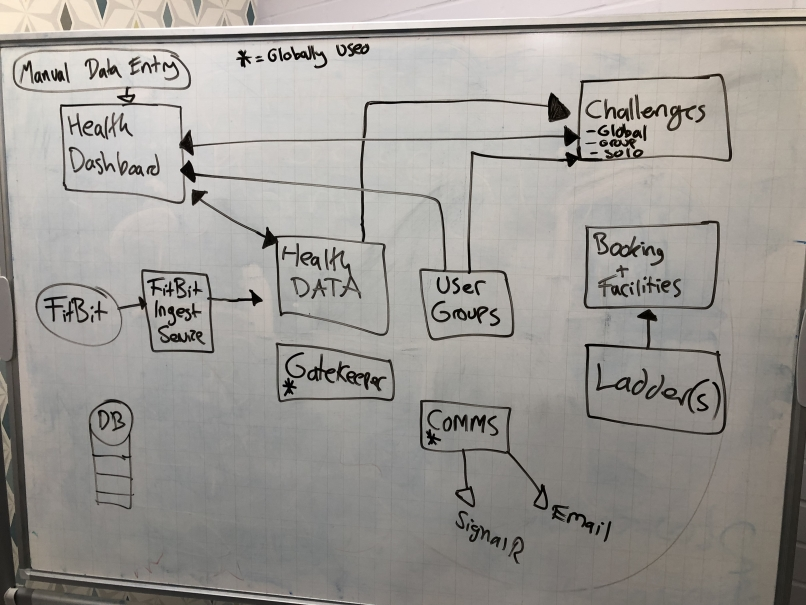
\includegraphics[width=\textwidth]{Images/Initial_Spec_Chart.jpg}
    \caption{An initial design diagram which was used to help break down the project into smaller microservices and gain a rough understanding how each microservice could interact}
\end{figure}

Once the individual microservices had been decided upon, we set out on allocating each microservice to two members of the team and assinging each service a priority ranking between 1 and 3, depending on how the services depended on one another. Services marked with a priority of 1 were core parts of the \textit{AberFitness} infrastructure on which many other parts of the system relied on their APIs in order to function correctly, such as the \textit{Health Data Repository} microservice.  \textbf{TODO: Link to figure below}

\begin{figure}[H]
    \centering
    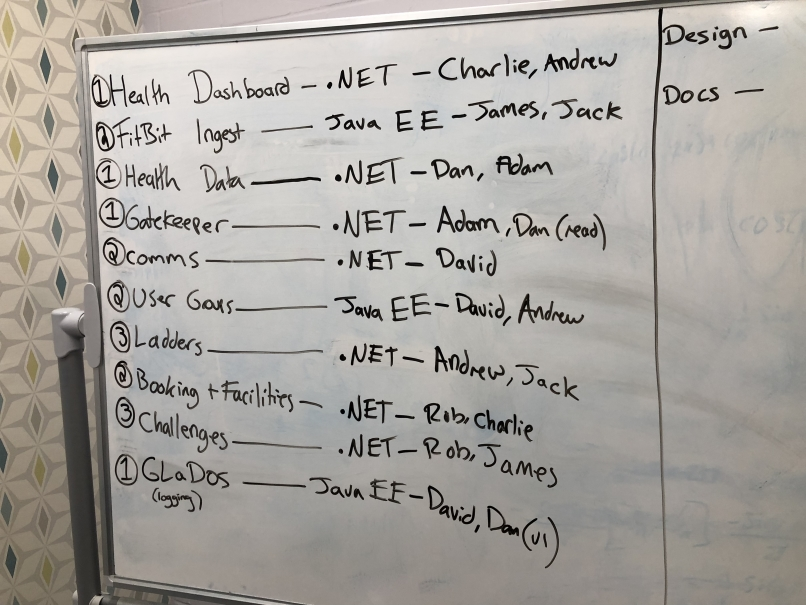
\includegraphics[width=\textwidth]{Images/Numbering_Microservices.jpg}
    \caption{Initial plan for ordering microservices in terms of priority and allocating them to members of the team for development}
\end{figure}


\section{Supporting Tools}
\subsection{GitHub \& TravisCI}
Each microservice for \textit{Aber Fitness} was hosted on \textit{GitHub}\footnote{https://github.com/sem5640-2018}. \textit{GitHub} provided many features which proved incredibly useful during the development phase, such as tight integration with \textit{Slack} for notifications straight to our chatrooms and integration with \textit{TravisCI} to automatically trigger unit tests and \textit{Docker} image builds. We also developed a development pattern of requiring all code to be peer reviewed through the use of pull requests and branch protection, a collection of settings which require that a series of conditions have been met before a pull request is able to be merged into the \textit{development} or \textit{master} branch. We configured branch protection in order to ensure that only tested, peer reviewed code would be committed into any upstream branch to reduce the likelihood of errors being introduced into the system and so that any issues could be caught early on. 

\begin{figure}[H]
    \centering
    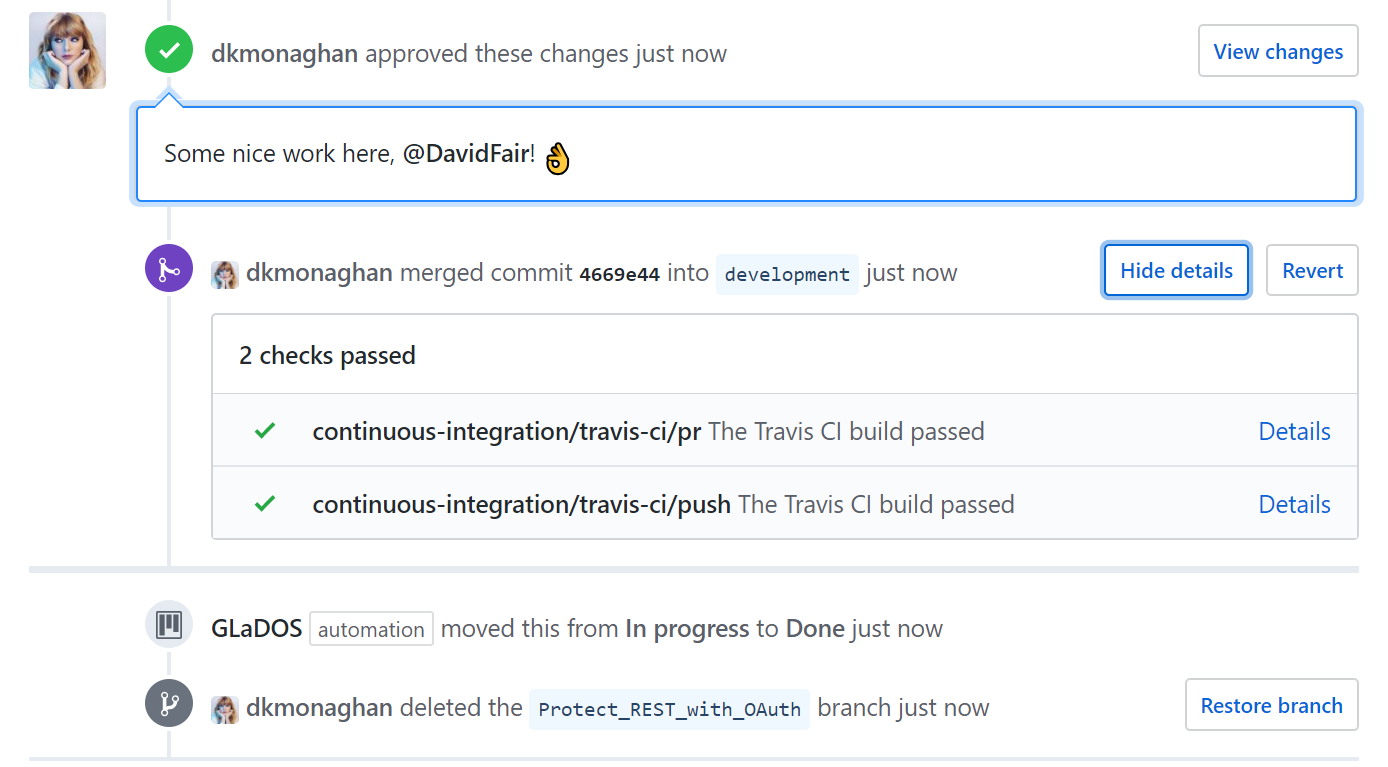
\includegraphics[width=\textwidth]{Images/approve_pr.png}
    \caption{A screenshot from \textit{GitHub} showing a pull request on the \textit{GLaDOS} repository being peer reviewed and also checks from \textit{TravisCI} passing before being merged into an upstream branch.}
\end{figure}

Once a pull request had been approved and merged, \textit{TravisCI} would then be responsible for building and pushing the \textit{Docker} image to \textit{Docker Hub}.

\begin{figure}[H]
    \centering
    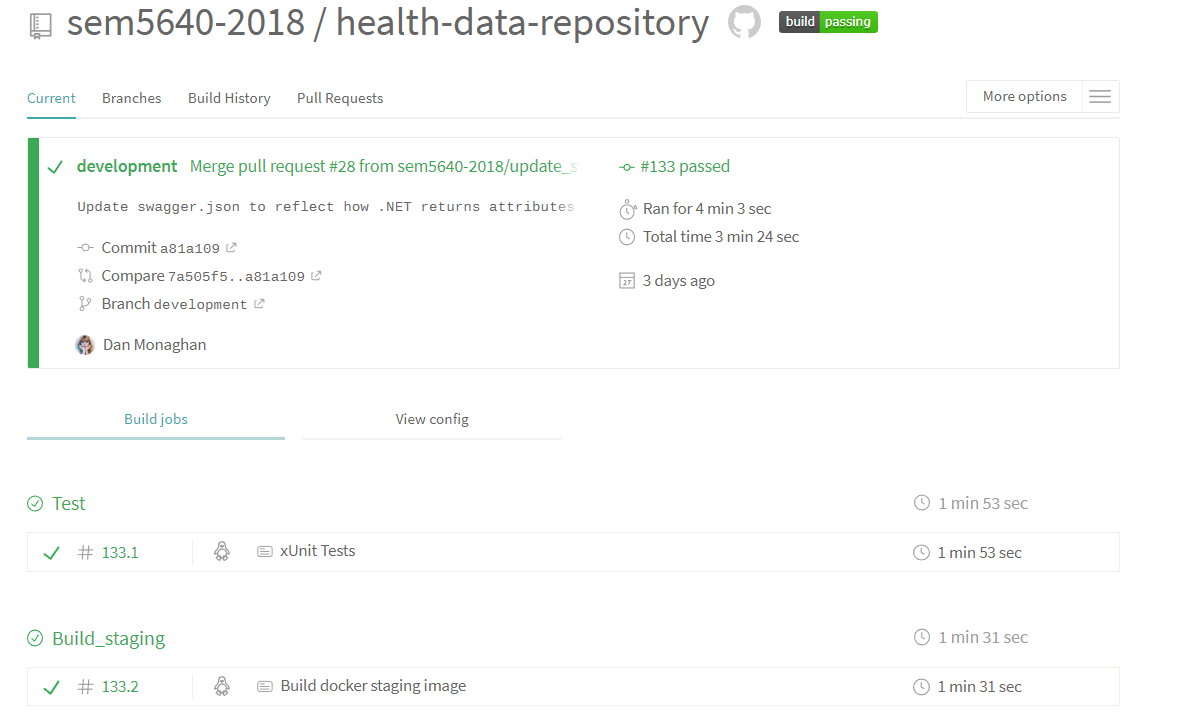
\includegraphics[width=\textwidth]{Images/travis_builds_overview.png}
    \caption{A screenshot from \textit{TravisCI} demonstrating a pull request being merged into the \textit{development} branch, re-passing unit tests once merged and then building the \textit{Docker} image}
\end{figure}

\subsection{Swagger}
\begin{figure}[H]
    \centering
    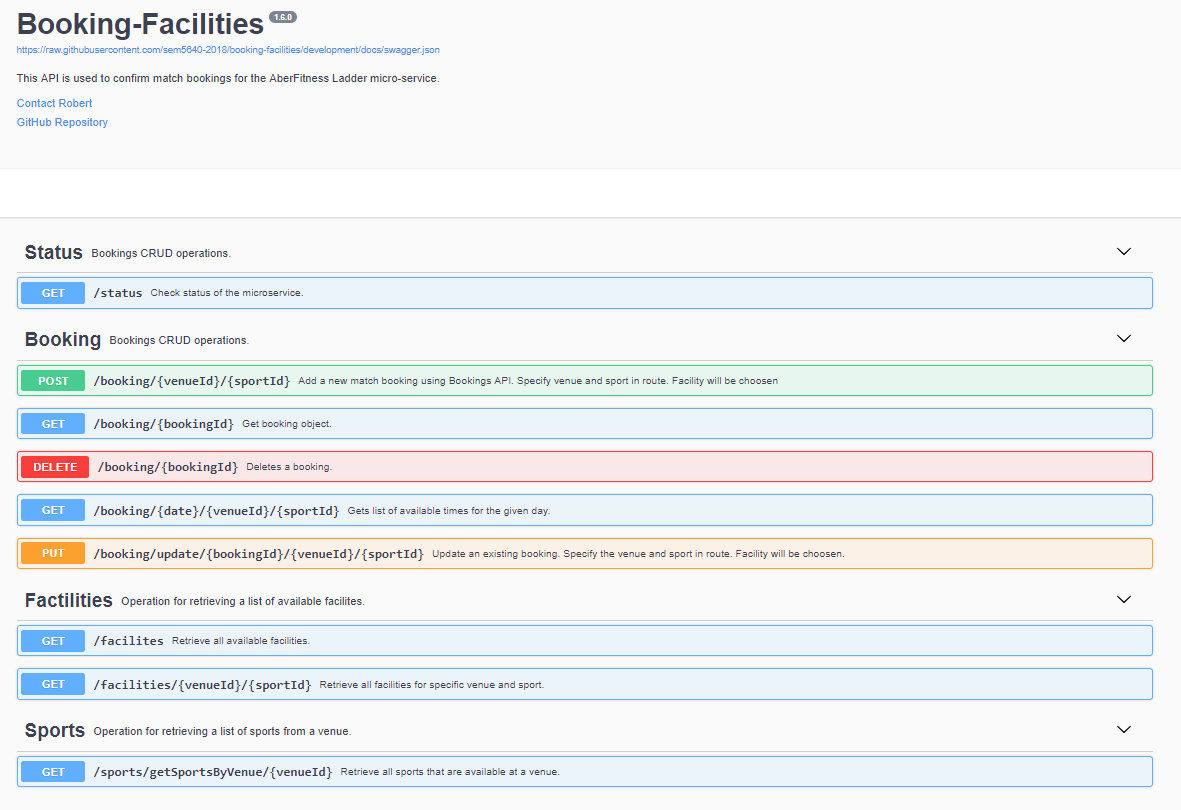
\includegraphics[width=\textwidth]{Images/Swagger.png}
    \caption{The Swagger interface for the \textit{Booking Facilities} microservice}
\end{figure}

\textit{Swagger} is a web based application for viewing API specifications. Each microservice within \textit{Aber Fitness} has a file located at \lstinline{docs/swagger.json} which defines its API endpoints and any associated data models. \textit{Swagger} was a crucial part of the development process as it allowed us to draft up API specifications prior to development in order to get feedback from other members of the group, and allowed issues to be identified early on in the event that a draft API specification lacked endpoints which would be required by other microservices. 


\subsection{Portainer}
\begin{figure}[H]
    \centering
    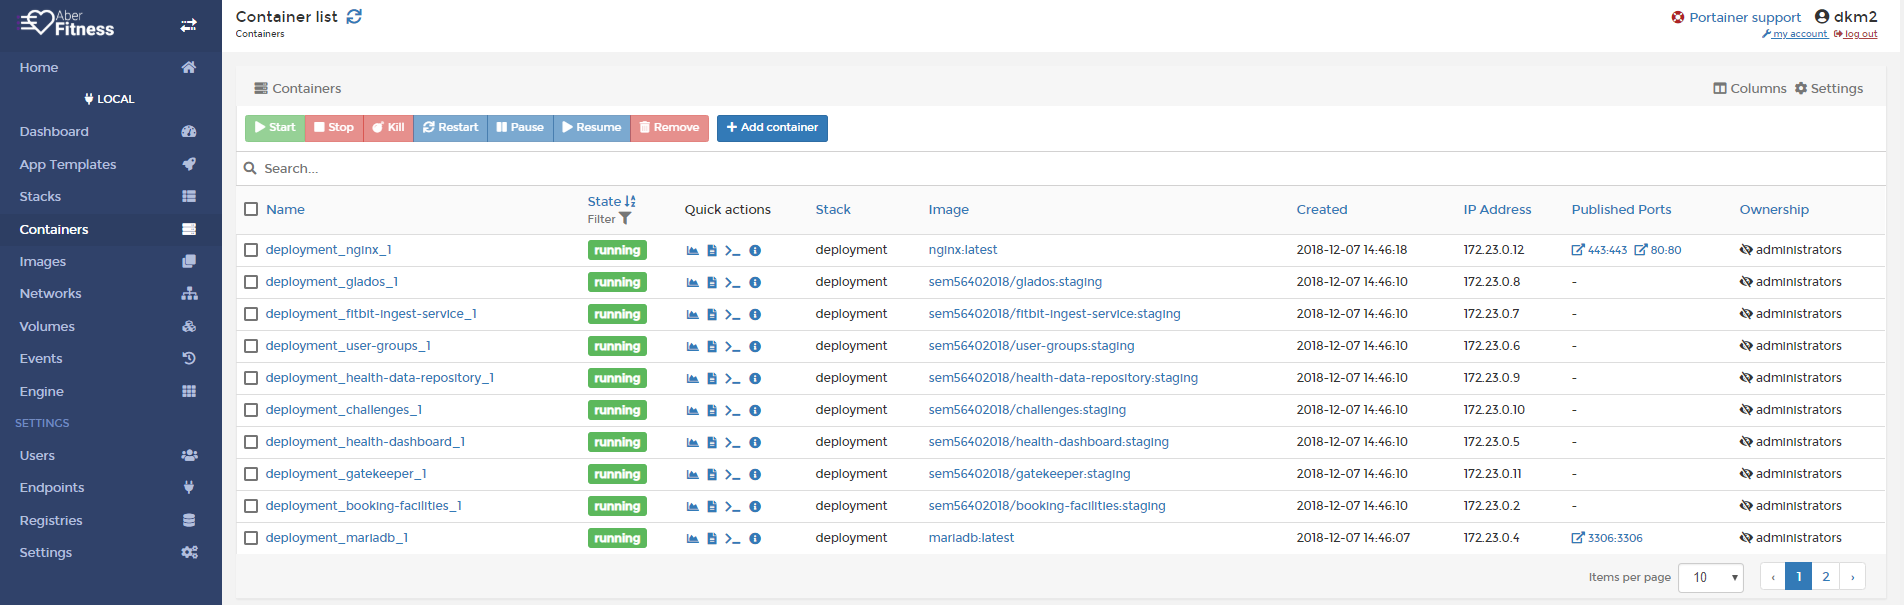
\includegraphics[width=\textwidth]{Images/Portainer.png}
    \caption{The Portainer interface for our staging / development Docker host, \lstinline{docker2-m56.dcs.aber.ac.uk}}
\end{figure}

\textit{Portainer} provides a dashboard for managing volumes, networks, images and containers on \textit{Docker} hosts. Throughout the initial configuration of the \textit{Docker} images, \textit{Portainer} proved invaluable as it provided the ability to quickly and easily understand what the host was running. \textbf{TODO: More here probably.}

\subsection{Docker Hub}
\textit{Docker Hub} is a platform provided by \textit{Docker} which allows \textit{Docker} container images to be uploaded and hosted, and easily pulled down by the \lstinline{docker-compose} script. As part of our build process (\textbf{TODO: reference build pipline diagram here}), images are built by \textit{TravisCI} and then pushed to \textit{Docker Hub} before being pulled down onto the \textit{Docker} hosts.


\subsection{Slack \& Deployment}
\textit{Slack} is an online text based chat service designed for offices and teams, and paticuarly suits itself to the development of software. The group used \textit{Slack} extensively throughout the development of \textit{Aber Fitness} not only to communicate and discuss progress, ideas and troubleshoot problems, but also made extensive use of \textit{Slack}'s integrations with services such as \textit{TravisCI} and \textit{GitHub}. 

\begin{figure}[H]
    \centering
    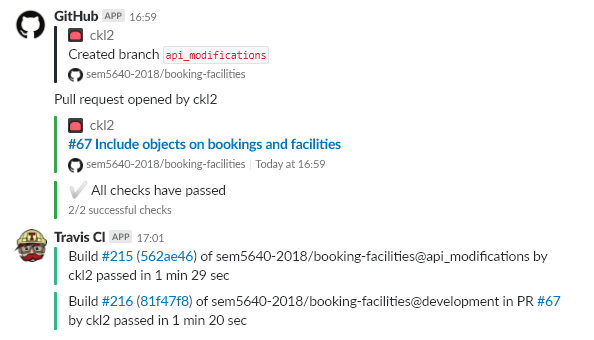
\includegraphics[width=\textwidth]{Images/Slack_Travis_GitHub.png}
    \caption{A screenshot of the \textit{Slack} channel \lstinline{\#dev-booking-facilities} demonstrating the integrations between \textit{Slack}, \textit{GitHub} and \textit{TravisCI}}
\end{figure}

\textit{Slack} also played a major role in our deployment strategy when rolling out updated \textit{Docker} images to our staging host. Due to the nature of the configuration of the two \textit{Docker} hosts we had been provided by the Computer Science department we ran into many issues with our deployment process, primarily to do with permissions on the host. Each member of the team had their own individual log in to the hosts, however we would frequently run into permissions errors when performing commands like \lstinline{git pull}. Other issues we had involved team members forgetting the specific set of commands which needed to be executed, wasting valuable development time. \textbf{TODO: figure no.}

\begin{figure}[H]
    \centering
    
\includegraphics[width=0.5\textwidth]{Images/aberfitness_slack_bot_reason_why.png}
    \caption{An example situation where the execution of \lstinline{docker-compose pull} caused a large amount of confusion amongst \textit{Aber Fitness} developers}
\end{figure}


\textit{Slack} ended up providing us with an elegant solution to this through its ability to easily call a webhook when a user typed a specific message in a chat channel. A quick \textit{Slack} application was put together to automatically pull the latest \lstinline{docker-compose.yml} file from GitHub, as well as updating all the \textit{Docker Hub} images, then re-deploying the stack. This could all be done from within \textit{Slack} itself through the \lstinline{/deploy} command. \textbf{TODO: Figure no.}

\begin{figure}[H]
    \centering
    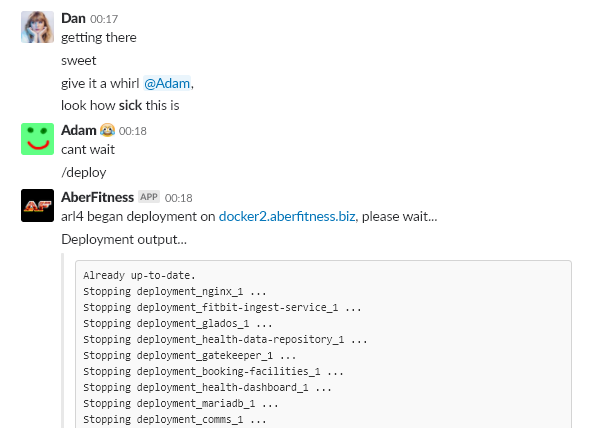
\includegraphics[width=0.9\textwidth]{Images/aberfitness_slack_bot.png}
    \caption{A demonstration of the \lstinline{/deploy} command being used to re-deploy \textit{Aber Fitness} onto the staging host}
\end{figure}


\chapter{Design}

\section{System Overview}
The \textit{Aber Fitness} system is broken down into a number of microservices in order to aid portability, scalability and promotes a more maintainable codebase. After reviewing the initial project specification, the following microservices were created:

\begin{itemize}

	\item \textbf{Booking \& Facilities} - The \textit{Aber Fitness} offers functionality for users to be able to schedule bookings at sports venues, such as swimming pools and squash courts. This microservice is called used by the \textit{Ladders} service to create bookings for competitions.

	\item \textbf{Challenges} - The system offers the ability to give users activity challenges, for example completing a number of steps in a specific timeframe. These challenges can also be 'group' challenges, where a number of users can compete against each another to achieve goals such as furthest distance walked in a week, etc.

	\item \textbf{Communications} - This microservice provides an API for other services to send email notifications to users. It does not present any form of web UI, and users do not directly interact with it. This system could also be easily expanded to send out text messages, push alerts, etc. depending on future requirements.

	\item \textbf{Fitbit Ingest Service} - At launch, the \textit{Aber Fitness} platform allows a user to link their \textit{Fitbit} accounts to the system in order to import their activity data. The service periodically polls the Fitbit API for new data on the users' behalf, then stores this into the \textit{Health Data Repository}.
	
	\par With the possibility of adding future platform support the "ingest service" concept was created. This would allow us to support services such as Apple's \textit{HealthKit} and other fitness tech providers. 
	This architectural design means that activity data can be normalised by a number of "ingest services" before being passed through to the \textit{Health Data Repository} service for storage. 

	\item \textbf{Gatekeeper} - \textit{Gatekeeper} is \textit{Aber Fitness}'s OpenID Provider, and handles all authentication within the system. User credentials and account metadata is stored within \textit{Gatekeeper}\textit{Gatekeeper} uses the OAuth 2.0 flow and is responsible for providing a single sign-on service for all of the various microservices. Microservices also contact \textit{Gatekeeper} to obtain and verify tokens when calling internal APIs.

	\item \textbf{GLaDOS} - \textit{GLaDOS} is the centralised auditing mechanism for \textit{Aber Fitness}. It presents a REST API which is used to store audit data; such as when a user's data was accessed, modified, or deleted. \textit{GLaDOS} also provides a Status page which displays the availability of all the other microservices.

	\item \textbf{Health Dashboard} - \textit{Health Dashboard} is the first interface users will encounter after logging in, or navigating to \textit{Aber Fitness}.  It provides the user with an overview of their recent activity as well as providing updates on any challenges or ladder competitions the user may be involved in.

	\item \textbf{Health Data Repository} - The \textit{Health Data Repository} service is responsible for providing an API for accessing and storing activity data. It receives normalised activity data from the Ingest Services, and provides multiple API endpoints for other microservices to access user activity data. 

	\item \textbf{Ladders} - \textit{Ladders} is responsible for organising and managing ladder style competitions among users of the system. Users can compete in sporting championships for a variety of competitive sports such as tennis, running or cycling etc. The \textit{Ladders} service also automatically books venues for upcoming competitive events, which is managed by the \textit{Booking Facilities} microservice.

	\item \textbf{User Groups} - \textit{Challenges} can also be turned into a competition amongst users of a group. For example, a group may consist of a few friends or an entire office department. Users within a group compete to complete goals, such as who can achieve the most steps in a single day. The \textit{User Groups} service is responsible for managing users into groups, and allowing users to leave and join other groups.

\end{itemize}

\subsection{Persistence}
    \par
    The system also required persistent database storage for all of the backend microservices to store activity data, user accounts, logs, and more. Every microservice would need to connect to a database instance.

    \par
    Object relational mapping \textit{(ORM)} is a technique for writing database-agnostic models and queries for persisting data. To keep code both testable and maintainable, both .NET Core and Java services use an ORM layer. Scaffolding subsequently generates database schemas based on the application's model classes

    \par
    \textit{MariaDB}\cite{MariaDB} in a Docker container was selected for several reasons. Firstly, the database provides data consistency guarantees when a record it persisted from the ORM layer. Secondly, native .NET core and Java connectors exist as public framework packages. Finally, the software is GPL licensed to avoid future issues with proprietary software, including alternatives such as Microsoft SQL.

\subsection{Model View Controller Pattern}
    \par
    All implementations use the Model-View-Controller \textit{(MVC)}
    pattern. This enhances testability by keeping constraints and functional logic within a model class. Controllers use an instance of the model and prepare data for return in a view. Dependency injection and reflection were used to test .NET core and Java components. These design patterns allow developers to replace concrete types with mocks at runtime based on the class interface.

    \par
    Additionally, the system was built with emergent design: using the MVC pattern with either dependency injection or reflection, depending on the langauge. Automated unit testing allows developers to refactor and re-organise their classes as more features were implemented.	

\subsection{Packaging}
    \par
    It was decided to use docker hub to deploy the images, these can be combined into an application stack defined in a \textit{docker compose} file. This also allows manual definition of internal networks, start-up order and filesystem volumes for each image.

    \par
    The deployed stack can be restarted or updated with the `\textit{docker-compose}' command, whilst individual containers can be managed using the docker commands directly. As part of the start-up process, volumes are mounted and environment variables are injected into the image.

\section{Integration}
\subsection{Authorization}
    \par
    The entire site is protected with the OAuth 2.0 token flow. Users login using a central authorization and receive a bearer token. This is send in the header of the request, as the user visits each microservice. As users persist their token locally between services this provides a seamless login experience.

\subsection{Internal Communications}
    \par
    To maintain compatibility between the various microservices a common messaging language was selected. Building on the groups experience writing web applications, we serialise messages into JSON and use REST APIs. These APIs can also be protected with the OAuth 2.0 authorization flow.

\subsubsection{Nginx}
    \begin{figure}[H]
        \centering
        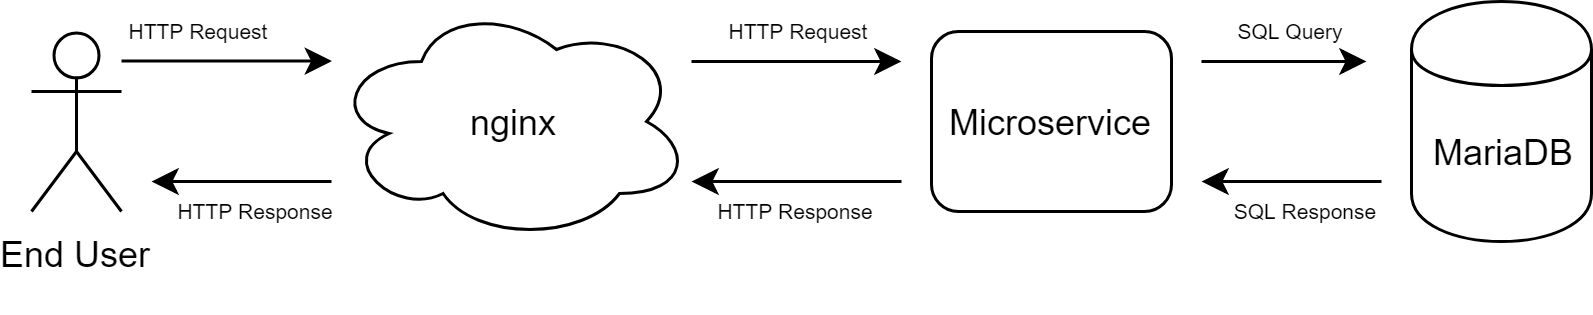
\includegraphics[width=\textwidth]{Images/nginx_proxy_flow.png}
        \caption{Traffic flow diagram showing an end user's browser connecting to the internet facing \textit{nginx} server, which then proxies requests through to the backend microservice}
    \end{figure}
    
    The Aber Fitness system architecture means that not exposed to the internet, but are instead available over an internal Docker network which allows containers to communicate with each other. In order to provide external access to the web servers of all of our microservices we have deployed nginx, an open-source and free web server which features highly customisable config files. Through the use of nginx's \lstinline{proxy\_pass} directive, we are able to take requests from end users and pass them through to the correct backend microservice based on the requested URI. \textbf{TODO: link figure above}
    


\chapter{Implementation}

\section{Deployment}

\section{Java EE}
    \subsection{Common Components}
        \subsubsection{Handling Dependencies and Static Analysis}
        \par
        At the start of the project the JavaEE development teams agreed to use \textit{Maven}\cite{Maven} to handle their dependencies. This allows the entire build process to be ran at the commandline rather than within the IDE, which is essential for \textit{TravisCI} integration.

        \par
        Maven uses an XML file called \textit{POM.xml} to define the dependency names, versions and additional options. These are fetched from Maven Central and cached locally for future builds. To add a new dependency a developer simply visits the hosting website and copies the XML provided alongside each package. Additionally developers can use the \textit{Scope} option which instructs the packaging plugin the associated \textit{JAR} files are provided by the Payara runtime.
        
        \par
        \textit{IntelliJ} natively supports reading from Maven's \textit{POM.xml} file, which defines the list of dependencies and compilation steps. Maven also contains a plugin which allows developers to package the built files into a web archive (WAR). This did have some caveats however; running 
        `\textit{mvn war:war}' would result packaging artefacts from the previous compilation, without compiling the current application. This could lead to confusion as new changes would no be reflected without `\textit{mvn compile war:war}'.

        \par
        Whilst working locally developers could still rely on IntelliJ's built in mechanism for packaging and deploying to a local Payara instance. This allowed for rapid development feedback and iteration without the overhead imposed by Maven.

        \subsubsection{Creating Docker Images}
        \par
        By utilising the ability to run the entire build process on the command-line with Maven we were able to quickly add Travis CI integration. This would clean compile the entire application, run the full \textit{JUnit} test suite and lastly package a WAR file.

        \par
        Initially we used \textit{CheckStyle} to also enforce coding style conventions. However the rules were over-specified. Additionally, unlike other formatting tools there was no option to emit a patch-file which allows developers to automatically fix-up many errors such as incorrect white space or formatting.

        \par
        The Java teams migrated to the \textit{PMD}\cite{PMD} static analysis tool: this warns about unused fields and variables, unsafe constructs,and dangerous coding patterns.
        The Maven test target was modified to run the \textit{PMD}\cite{PMD} static analysis tool before any unit tests. If any violations were detected the build would immediately stop, ensuring all modifications were inspected.

        \par
        The groups proceeded to add a \textit{Dockerfile} to build a docker image for later deployment. Payara provide multiple images on \textit{DockerHub}\cite{DockerHub_Payara}, which range from the full server to an embedded instance.

        \par
        Initially we copied the local web archive, which was built on Travis, into the full Payara deployment folder. This allowed us to use the web administration console to resolve various deployment issues without having to dig through log files. After moving changing the default source code layout, which resolved \textit{resources} not being included in the final archive, we successfully deployed GLaDOS to the full instance.

        \par
        However we could not get Fitbit Ingest to successfully deploy, they had already started implementing the OAuth flow which is required by both the Fitbit API and our own internal API. The internal SSL implementation had changed with JDK update 191, which prevented the \textit{CDI} layer from initialising the associated beans.

        \par
        As the bundled JDK version is controlled by Payara in the base image we proceeded to look for an alternative solution. We decided against modifying the image to transplant a specific JDK at build time. Instead, we found that there was an open upstream issue\cite{payara_ssl_issue} that used reflection to resolve the problem internally. As this fix was not released into the latest stable release we had to switch to running pre-release images for all Java EE applications.

        \subsubsection{Migrating to Micro Image}
        \par
        The Payara Microprofile image is designed specifically to be used in Docker deployments. Whilst this does not implement the full EE, the memory usage is ten times lower at 90MB. The profile still provided the required set of services for the application so there was a significant benefit to completing this migration. However trying to deploy to the micro instance resulted in an exception being thrown whilst completing the implicit bean discovery phase. 

        \par
        The CDI 1.1 specification and above requires the server to automatically scan for injection points and pair it with matching enterprise Java beans (EJBs). This can fail with older dependencies, so we initially suspected one of the dependencies did not correctly use the \textit{beans.xml} annotation to turn this off.
        \newline
        Switching off bean discovery and manually annotating them allowed the ingest service to correctly deploy. However bean discovery is required for Facelets 4.0 and an exception will be thrown if it is not enabled. A new project was created with all but the essential dependencies removed, and we discovered the exception was still thrown which only added to the confusion. 
        
        \par
        By looking at the package namespaces associated with the injection points and running `mvn dependency:tree' we could see that `\textit{org.sonatype.guice}' was the culprit. Walking up the tree we discovered that the WAR plugin was being included in our packaged dependencies. At deployment the microprofile server tried to start a Maven instance and failed, thus removing this dependency correctly allowed the application to start. The development teams realised that the plugin was included in our installed copies so we could still continue to use it.

        \label{JTA_Targets}
        \subsubsection{Setting up JTA Targets}
        Both services started off by instantiating the single JDBC connection through the driver manager as required. This had some caveats however: Firstly, the JDBC driver had to be distributed and managed within the web archive. Secondly, there was no form of connection pooling to allow for scaling at the persistence layer.

        \par
        Traditionally a connection pool is created using the administration web GUI. However this would require a developer set up the pool each time continuous deployment finished on a full instance. The microprofile we had just switched to did not provide a web GUI at all.

        \par
        Glassfish allows a web application to specify resources found on the server using `glassfish-resources.xml'. This XML file can also use system environment variables allowing us to protect and specify database credentials on the deployment targets. The examples found online primarily pertained to a \textit{MySQL} deployment, so multiple iterations of testing and deployment were required to get the pool working successfully. This switch allows an application to detect and create connection pools at deployment, allowing the images to rapidly redeploy facing another database instance.

    \subsection{Fitbit Ingest Service}
        \subsubsection{To Do}

    \subsection{GLaDOS}
        \subsubsection{REST API}
        \par
        The primary role of GLaDOS is to store audit data so that users can view how their data was viewed and modified. Whilst there are native implementations, such as the Java Messaging Service, these require the calls be proxied into a local JVM instance to handle the transport component. We chose to serialise into JSON and use REST as the transport mechanism as all applications had native support for this set up.

        \par
        \textit{JAX-RS} is an API specification for JSON parsing in Java, additionally Payara provides \textit{Jersey} as the implementation of this API at runtime. This avoided us having to package additional dependencies into the web archive. This also allows us to build standard response pages based on the error code internally generated, avoiding having to develop error views.        

        \subsubsection{Unit Testing and Mocks}
        \par
        A new class abstracting the database layer allowed us to avoid writing entity handling at this. We instead focused on writing unit tests which verified the various endpoints correctly serialised or de-serialised data. \textit{Mockito}\cite{Mockito} allows developers to inject mock objects by specifying the class which the test fixture is using.

        \par
        We could not use dependency injection within the endpoint implementation, as the instantiation point is internal to the framework. This doesn't prevent us from using mocks as Mockito allows a developer to inject them through the reflection methods built into the library. A database call such as `\textit{db.getEntry(id)}' could be tested to see which status codes would be sent and verify the data,if any, was serialised correctly.

        \subsubsection{Integration Testing with Arquillian}
        \textit{Arquillian}\cite{Arquillian} allows developers to specify the classes to archive and deploy within the text fixture. Payara also provides an embedded Arquillian test container which can be ran at test time to exercise sections of a full system. This would allow us to write integration tests for an end-to-end operations, such as POSTing data to an endpoint and ensuring it is written to the persistence layer.

        \par
        There was extensive documentation on the methods required to pack an archive, but limited examples on handling Maven dependencies. As the embedded instance provides no runtime methods we were having problems getting the container to correctly run. Developers could specify the full class paths for their dependencies to ensure the were packaged, but this was extremely verbose and fragile.

        \par
        We looked into using the Maven dependency resolver, which allows developers to get a list of runtime Jars and package them into the archive. However this would led to another set of problems where Maven was trying to export them into a \textit{.zip} format, then throw an exception because this was not supported.

        \par
        With no easy was to control the format that runtime dependencies were exported in, combined with a lack of documentation pertaining specifically to Maven we agreed to abandon this method of automated testing. This would give us more time for implementing other components within the deadline. We opted to rely on manual integration testing for the duration of the project instead.

        \subsubsection{Entity Management}
        This service only persists Audit Data, therefore we ultimately need to persist a single entity. Whilst many ORM solutions exists for Java, such as \textit{Hibernate}, we decided against them due to the implementation overhead that was required.

        \par
        Instead we relied on the persistence layer provided in the EE specification. Using the connection pools which were set up for both Java services (see \ref{JTA_Targets}), we could specify which JTA the injected entity manager should use.

        \par
        The table schema is managed through annotations on an entity class. This also allows the implementation provided by Payara, \textit{EclipseLink}, to create the tables required at deployment time. As the framework relies on the field types to determine which underlying storage to use there is a hidden pitfall. If the type does not have a native serialisation Java will try to persist this using binary data.

        \par
        Instants are used to specify timestamps on logs, these are cross compatible as they use \textit{ISO 8601}\cite{ISO_8601}, a string specifier for absolute time points. This format allows both .NET Core and Java application to send timestamps in the following format \textit{2018-11-28T12:04:14Z}. However as this type was added in JDK 8 there is no native storage conversion built into the entity framework.

        \par
        Two adaptors were written based on the \textit{AttributeConverter} interface. These provide methods for marshalling and un-marshalling Instants into String objects, which the entity manager can easily store. Annotating the field installed the converting class and correctly updated the schema. This also has the added benefit of making the stored timestamps human readable within the database, which extremely helpful for debugging.

        \subsubsection{Developing Facelets}
        \par
        GLaDOS also provides a page that allows a user to retrieve audit data associated with their account. Administrators can look up any users audit data by user their unique ID too. In addition there is a status page which allows anyone to view the status of all other micro-services without logging in.

        \par
        The front-end of GLaDOS use facelets to implement the MVC pattern. A backing bean for the user data uses named queries from the persistence layer to retrieve data into a list of entity objects. We switched to using \textit{PrimeFaces}\cite{Primefaces}, which is a fork of the now deprecated \textit{RichFaces}. This allows us to use components such as \textit{DataTables} which dynamically generate tables based on the number of entries returned.

        \par
        The Fitbit Ingest Service had completed OAuth implementation for connecting to internal and external APIs. This was ported across to GLaDOS and further modified. As the ingest service has no front-end they don't need to persist \textit{JSON Web Tokens (JWTs)}. Additional methods were written specifically for this microservice. These include using the HTTP session handling built into the web framework to persist the token on the server. Another helper class was written which validates the stored JWT as the user navigates through protected pages, or POSTs any requests.

        \par
        Service statuses were implemented using a singleton Java bean which is instantiated at deployment. Using the scheduling capability provided for EJBs we poll all services every 20 seconds in a seperate thread. All services implement an endpoint at \textit{/api/status} that returns a 200 or 204. This is stored until the page is retrieved where the backing bean, acting as a presenter forward the results on.

        \par
        As the application stack uses an \textit{nginx} instance to reverse proxy queries the URLs must take this into account when they are generated within the facelet. .NET Core makes this trivial by calling `\textit{App.UsePathBase(URL)}' at start up, however Java applications rely on the context root. This was interfering with the URL rewriting that Nginx performs resulting in the service using the 
        `\textit{/glados/glados/}' base path.

        \par
        Initially we used an environment variable to manually generate links between the pages of the service and set the context root to 
        `\textit{/}'. However, this quickly proved to be untenable when using forms, as POST requests were being sent to 
        `\textit{/destination}' 
        rather than 
        `\textit{/glados/destination}'. Ultimately to work around this an exception was added to Nginx configuration to avoid re-writing any URLs for GLaDOS, and instead rely on the service to correctly address all requests. This allowed us to switch back to generating addresses based on the \textit{outcome} tag and use forms on the service.



\section{.NET Core}
    \subsection{}{Common Components}
some blurb about .net core here

    \subsection{Booking Facilities}

    \subsection{Challenges}

    \subsection{Communications}

    \subsection{Gatekeeper}

    \subsection{Health Data Repository}

    \subsection{Health Dashboard}

    \subsection{Ladders}

    \subsection{User Groups}

\chapter{Testing}
\par
One of the core tenets of continuous deployment is the reliance on a mix of automated and manual testing to ensure a system is functioning correctly. The applicable subset of these tests were run before each change specified in a pull request was accepted. The full suite was run as part of the release process, which allowed developers to deploy the application to production with confidence.

\section{Unit Testing}
\par

\par
\subsection{Framework Choices}
\textit{.NET Core} and \textit{Java EE} both have a host of unit testing frameworks to choose from. In order to maintain consistency, it was decided that the a single framework would be used for all \textit{.NET Core} applications and another single framework for every \textit{Java EE} application. The development teams agreed on using \textit{xUnit}\cite{xUnit} for .NET Core, and \textit{JUnit}\cite{JUnit} for \textit{Java EE} early into the project.

\par
For \textit{.NET Core} applications, xUnit was chosen in place of \textit{MSTest} and \textit{NUnit}. Recent documentation and examples from Microsoft have focused on xUnit instead of MSTest. xUnit is significantly more extensible through the use of the \textit{Theory} attribute, allowing a single test method to be written for multiple datasets.

\par
Additionally, xUnit extends upon principles found in NUnit with additional features, such as the ability to execute individual test methods\cite{Nunit_XUnit_comparison}. It also instantiates a new test instance for each fixture, ensuring that side effects do not propagate through a test suite. This prevents problems with ordering tests found in some software projects.

\par
JUnit is an almost ubiquitous testing framework for \textit{Java EE} for a few reasons; it has strong integration with other tools, such as Maven and various mocking frameworks, and documentation is widely available. Multiple versions exist so the \textit{Java EE} teams chose to use version 5, as it is the latest stable release on JUnit.

\subsection{Mocking}
\par
\textit{Moq}\cite{Moq} is used for mocking injected dependencies in \textit{.NET Core} services. Classes were written using the dependency injection pattern, accepting a concrete type at construction time. Using Moq objects is extremely simple; developers instantiate their mock based on an interface, then set up expectations, if any, and verify the calls.  The library also allows developers to provide mock implementations of methods available on the interface to enable more in-depth testing of the component.

\par
\textit{Java EE} requires a slightly different approach, as an EJB cannot have arguments in its constructor. \textit{Mockito}\cite{Mockito} provides an alternative to dependency injection; developers create fields in the class which match the types which are constructed in the EJB. These are annotated with `\textit{@mock}' and subsequently injected with `\textit{@injectMocks}' on the test instance. Mockito supports \textit{Hamcrest}\cite{Hamcrest} matchers which were also used to handle more complex assertions.


\section{Integration Testing}
\par
Most of the micro-services provide internal APIs, which are not designed for external usage. To protect these endpoints the OAuth 2.0 flow was used to authorize application interactions with client credentials. Whilst unit testing ensures each API correctly responds according to its documented behaviour, it does not exercise all components that partake in an interaction.

\par
As REST endpoints were used as the primary message exchange method we could send and request JSON payloads to ensure the system under test behaved as expected. Multiple third party solutions were used for testing APIs, \textit{Postman}\cite{Postman} was one instance that was widely used by the development team. 
This can handle the OAuth flow 

\par
Developers used these tools to ensure that malformed requests or interaction with no authorization token were correctly handled. Additionally they can handle the OAuth flow on a developers behalf, this was extremely useful when debugging interactions between applications and resolving digressions from the API specifications.


\section{System Testing}
\par
Aber Fitness was deployed onto two separate \textit{Docker} hosts, representing staging and production. Developers could trigger a deployment from the latest development images in \textit{Slack}, and then manually test the system in a deployed state. This also allowed for the detection of deployment specific problems, which are un-testable without a complete system.

\par
One example of an issue caught by manual system testing was within the \textit{Challenges} microservices, which contained a controller which was not operating asynchronously. Unit tests would not exercise the instance in parallel, so this bug was not caught in unit testing. The bug resulted in API calls made to the deployed application returning a HTTP 502 response, due to the original call putting the controller in a blocked state and preventing it from responding to the next call.


\section{Static Analysis}
\subsection{PMD}
\par
Initially, Java used \textit{CheckStyle} to also enforce coding style conventions. However, the rules were far too strict to be beneficial or practical and, unlike other formatting tools, there was no option to emit a patch-file which allows developers to automatically fix-up many errors such as incorrect white space or formatting.

\par
The Java teams later migrated to the \textit{PMD}\cite{PMD} static analysis tool: this warns about unused fields and variables, unsafe constructs, and dangerous coding patterns.
The Maven test target was modified to run the PMD static analysis tool before any unit tests. If any violations were detected the build would immediately stop, ensuring all modifications were inspected.

\section{Acceptance Testing}
\par
During our first meeting, the project's functional requirements were broken down into a number of spreadsheets, each based on the service which would implement them. The client was then contacted to clarify any requirements which were ambiguous to the group. Acceptance tests for each micro-service were added to a spreadsheet based on these original and revised requirements.

\par
Acceptance tests are completed manually by completing the steps defined by the document. Each test is marked as pass or fail based on the criteria also set out in the document, allowing the individual microservices, and by extension the entire project, to be assessed on its fitness for purpose.

\par
A fresh deployment of the system was performed shortly after a code freeze and the full suite of acceptance tests were completed. This round of testing highlighted 23 instances where the implementation deviated from the client's requirements.

\par
Bugs were assessed on a case-by-case basis, taking account of the impact. Fixes which had a low potential for regression and addressed high impact problems were implemented and merged after the code freeze. This process resolved 11 of those implementation issues, resulting in almost half of the failed acceptance tests becoming passes in the space of a few hours, and with no additional issues appearing as side-effects. This shows that internal acceptance testing was a highly valuable process that resulted in a noticable improvement in the final product.


\chapter{Status}
\chapter{Evaluation}

\section{Development Methodology}

  \subsection{Evaluation}
  \par
  The group met for weekly meetings at the start of the project to define a top-level system design on a whiteboard. These sessions were initially productive, as work was distributed to subteams and a unified approach for the various microservices was decided. As the project went on, the usefulness of these meetings was questioned. Attempts to design by committee would rapidly devolve into either a few interested parties talking about a single service, or every developer inputting an opinion on simple decisions.

  \par
  A vote unanimously agreed to change the group meeting into a session where every developer would work on implementation in the same room instead. This refocused teams onto their own design, whilst allowing an individual to still propose system-level questions or ideas in person. Productivity also rapidly increased as knowledge of common problems and solutions were shared amongst the group.

  \par
  Throughout the project there have been instances where the requirements were not clear. Reasons ranged from multiple interpretations, noun and verb conflation, and insufficient detail. Slack was used as a communication mechanism with the client, which allowed the client to choose an appropriate time to respond to requests, which could be sent at any time, while also enabling real time discussion. These communications taking place over a recorded medium meant that an answer could easily be converted into an additional requirement later.

  \par
  As the project progressed, Scrumban-related processes were skipped increasingly. Project boards weren't being updated or tracked and work was completed without an associated issue or project board entry. As there were eight members of the group, it became increasingly difficult to track the work that individual teams had remaining. Ultimately this lead to deadlines being missed, as teams had to estimate their work left to complete rather than having a metric to rely on.

  \par
  As the scope of each unit's work was not defined, branches would often contain multiple features and fixes. Pull requests would often alternate between being too large to sensibly review, or a single fix spread across several pull requests. Additionally, developers would typically review within a subteam, instead of examining other services' code. This lead to code reviews being approved without the approver properly reviewing the change. This culminated into several simple bugs and version control issues, which would likely have been spotted, such as incorrect equality comparisons being merged into the codebase.


\section{Future Improvements}

- \\TODO Blocked on status

- Integration Testing

\section{Fitness for purpose}
    \subsection{Functional Requirements}
    \par
    Based on the client's criteria we have fulfilled the majority of functional requirements, as seen in \ref{Requirements_chpt}. This was measured using acceptance tests which give a rough indication of conformity to the requirements. \\TODO tests were performed with \\TODO failing, giving a \\TODO \% final pass rate.

    \subsection{Design Constraints}
    \par
    Our application stack makes use of both Java EE and .NET Core, as per the design constrains. These languages also provide access to many frameworks and third party implementation through Nuget and Maven. 
    
    \par
    By carefully checking the license of all external code and finding alternatives where required, the system is completely free of proprietary software and licensing considerations. Additionally, this reliance on external packages for core components,such as \textit{Identity Server} for authorization, reduces the sites future maintenance overhead.

    Finally, deployable docker images were created for each microservice which ran on the destination server. This would also allow the system to scale the number of instances based on an individual service's load in the future.


\end{thebibliography}

\end{document}
